\documentclass[oneside, 12pt, a4paper]{book} %文章类型是book
						%使用xelatex编译
%\usepackage[Bjornstrup]{fncychap}
\usepackage{xltxtra,fontspec,xunicode}
\usepackage[BoldFont]{xeCJK}
\usepackage[usenames,dvipsnames]{xcolor}
\usepackage{tikz,ifthen}
\usepackage{longtable}
\setCJKmainfont[BoldFont=方正特雅宋_GBK]{方正准雅宋_GBK}	%使用宋体
\setmainfont{Arial}
\XeTeXlinebreaklocale "zh"
\XeTeXlinebreakskip = 0pt plus 1pt %设置中文自动换行

\renewcommand{\baselinestretch}{1.5} %正文行距
\usepackage{titlesec}
\newcommand{\sectionbreak}{\clearpage}

\usepackage{hyperref}%超链接

\usepackage{xcolor,graphicx}%插入图片
\usepackage{float}

\usepackage{geometry}%页间距
\geometry{left=2.5cm,right=2.5cm,top=2.5cm,bottom=2.5cm}
\raggedbottom

\makeindex


\title{图灵的礼物}
\author{09 SEers}
\date{June, 2013}


\titleformat{\chapter}[display]  %Chapter格式
  {\bfseries\Large}
  {\filright \chaptertitlename \Huge \thechapter}
  {1ex}
  {\titlerule\vspace{1ex}\filleft}
  [\vspace{1ex}\titlerule]

\titleformat{\section}[display]
  {\bf}
  {}
  {8pt}
 {\titlerule \vspace{1ex} \filcenter}
  [\vspace{1ex}\titlerule]

\titleformat{\subsection}
  {\bf}
  {}
  {12pt}
  {}
  [\vspace{1ex}]

\renewcommand{\contentsname}{目~录} %中文目录名

\setlength{\parskip}{1em}

\setlength{\parindent}{2em} %段落开头空两行

\usepackage{indentfirst}
\setcounter{tocdepth}{1}  %目录深度为2
\begin{document}
\clearpage
%% temporary titles
% command to provide stretchy vertical space in proportion
\newcommand\nbvspace[1][3]{\vspace*{\stretch{#1}}}
% allow some slack to avoid under/overfull boxes
\newcommand\nbstretchyspace{\spaceskip0.5em plus 0.25em minus 0.25em}
% To improve spacing on titlepages
\newcommand{\nbtitlestretch}{\spaceskip1em}
\pagestyle{empty}


\begin{figure}[h]

\includegraphics[width=4cm,height=2cm]{0cover/icons.eps}
\end{figure}\par

\begin{center}
\bfseries
\nbvspace[3]
%\Huge
%{\nbtitlestretch  \fontsize{36pt}{2}\selectfont 图灵的礼物}

%\nbvspace[1] 
%\fontsize{20pt}{15pt}\selectfont 南京大学~飞跃手册

%\small BY\\
%\small 09~SEers\\

\begin{tikzpicture}

    \coordinate (A) at (0,0);
    \coordinate (B) at (-60:6cm);
    \coordinate (C) at (240:6cm);
    \foreach \density in {20,30,...,160}{%
        \draw[fill=MidnightBlue!\density] (A)--(B)--(C)--cycle;
        \path
             (A) coordinate (X)
          -- (B) coordinate[pos=.15](A)
          -- (C) coordinate[pos=.15](B)
          -- (X) coordinate[pos=.15](C);

    }
\end{tikzpicture}

%\footnotesize You got a dream, you gotta protect it.


\nbvspace[3]
\normalsize
\begin{tikzpicture}[remember picture, overlay]
    \usetikzlibrary{calc}
	\draw[draw=none,fill=MidnightBlue!20] (current page.south west) rectangle
		($(current page.south east)+(0,3.5\paperheight/10)$);
	\draw[draw=none,fill=MidnightBlue!30] (current page.south west) rectangle
		($(current page.south east)+(0,1.3\paperheight/10)$);


	\draw[anchor=center] ($(current page.south west)+(0.5\paperwidth,  7\paperheight/10)$) node[yshift=0.5em]
		{\textcolor{black}{\fontsize{44pt}{2}\selectfont 图灵的礼物}};

	\draw[anchor=center] ($(current page.south west)+(0.5\paperwidth,  7\paperheight/10)$) node[yshift=-4.5em]
		{\textcolor{black}{\fontsize{20pt}{2}\selectfont 南京大学~软件学院}};

	\draw[anchor=center] ($(current page.south west)+(0.5\paperwidth,  7\paperheight/10)$) node[yshift=-7em]
		{\textcolor{black}{\fontsize{16pt}{2}\selectfont 飞跃手册}};

	\draw[anchor=center] ($(current page.south west)+(0.5\paperwidth,  3\paperheight/10)$) node[yshift=-4em]
		{\textcolor{white}{\Large "You got a dream, you gotta protect it."}};

\end{tikzpicture}
%July, 2013\\
%\large
%PUBLISHED AT NANJING
%\nbvspace[1]
\end{center}
\clearpage
\newpage
\clearpage
\begin{center}
\topskip0pt
\vspace*{\fill}
\Huge 图灵的礼物 \\
\vspace{3em}
\large BY \\
\large 09 SEers \\
\vspace*{\fill}
\vspace*{\fill}
\large July, 2013\\
PUBLISHED AT NANJING\\
\vspace*{\fill}
\fontsize{12pt}{2}\selectfont 版权声明: \href{http://creativecommons.org/licenses/by-nc-nd/3.0/cn/}{署名-非商业性使用-禁止演绎 3.0 中国大陆 (CC BY-NC-ND 3.0 CN)}\par
\fontsize{12pt}{2}\selectfont \copyright~2013 南京大学软件学院~~保留所有权利。
\end{center}
\clearpage
\newpage

\begin{center}
\topskip0pt
\vspace*{\fill}
To my dear Yolanda -- we sow in the fall,\\
Irrigate in the winter, and harvest in the spring.\\
We are the blessed children.
\vspace*{\fill}
\vspace*{\fill}
\end{center}
\clearpage
\addcontentsline{toc}{chapter}{目录}
\pagenumbering{roman}
\tableofcontents
\chapter*{序言}
  \addcontentsline{toc}{chapter}{序言}
\pagestyle{plain}
\chapter*{编者记}
  \addcontentsline{toc}{chapter}{编者记}
\pagestyle{plain}

GRE的一份真题材料叫作唐僧的礼物,因此当我有了整理一本小册子的想法的时候,本书的书名就跑到了脑海里面。回忆起那段和G奋斗的时光,算是大学里最静下心来做事的一段时间。就以这个名字,纪念我们都已度过,你们也终将度过的大学四年吧。\par
当初看完《上海交通大学学生生存手册》之后,内心的一些疑问得到了解答。因此立志在大学结束的时候,也要和伙伴们写出这样一本书。可惜当提笔的时候,却发现自己想说的很多话,都已在生存手册中讲过了。于是乎,只好罢笔。\par
后来,随着自己看到的世界越来越大,觉得定下一种模式其实是在限制自己。四年的生活,哪能仅仅归结于出国、保研、考研或是工作那么简单?所以此书虽以这四个方向来总结大家的结果,但也仅仅只能算是阶段性的报告。出国的人会回来工作;工作的人也可能到国外读研。正如默存先生那句名言:“城里的人想出去,城外的人想进来。”任何时间,你都有权利作出自己的选择。\par
最后讲一个不是很好笑的笑话吧:一个犹太人在一条路上建了个加油站发财后,后面跟来的犹太人建了理发店、餐厅、洗车房。一个中国人在一条路上建了个加油站发财后,后面跟来的中国人建了第二个加油站、第三个加油站、第四个加油站。
\chapter*{录取结果}
  \addcontentsline{toc}{chapter}{录取结果}
\pagestyle{plain}
\newpage
\begin{center}
\begin{longtable}{|c|c|c||c|c|c|}
\caption{美国CS录取统计}\\
\hline
\textbf{学校} & \textbf{Master} & \textbf{PhD} & \textbf{学校} & \textbf{Master}  & \textbf{PhD} \\ \hline
Brown & 1  & ~ & Stanford & 1 & ~ \\ \hline
Clemson & 1  & ~ & SUNY-Buffalo & 4 & 1(AD) \\ \hline
Columbia & 3 & ~ & SUNY-StonyBrook & 4 & ~ \\ \hline
Cornell	& 2 & ~ & Syracuse & 2 & ~  \\ \hline
CU-Boulder & 2 & ~ & TAMU & 5 & ~ \\ \hline
CWRU & ~ & 1(Offer) & UC-Boulder & 2 & ~ \\ \hline
Dartmouth & 2 & ~ & UCD	& 2	& ~ \\ \hline
Gatech & 1 & ~ & UCI & 5	& ~ \\ \hline
GWU	& 1 & ~ & UCSB & 1 & ~ \\ \hline
KU & 1 & ~ & UCSD & 5 & ~ \\ \hline
NCSU & 1 & ~ & UMich & 2 & ~ \\ \hline
NEU & 3 & ~ & UPenn & 2	& ~ \\ \hline
NYU	& 1 & ~ & USC	& 1	& ~ \\ \hline
OSU	& 3 & ~ & UT-Austin & 2 & ~ \\ \hline
Rice & 3 & ~ & UTD & 2	& ~ \\ \hline
RPI & 1 & ~ & UW-Madison & 1 & ~ \\ \hline
Rutgers & 1  & ~ & VT & 1 & ~ \\ \hline
SIT	& 1 & ~  & WPI & 2(1TA) & ~ \\ \hline
\end{longtable}

\begin{longtable}{|c|c|c|c|c|}
\caption{其他地区CS录取结果}\\
\hline
\textbf{学校} & \textbf{Master} & \textbf{Master Detail Info} & \textbf{PhD (Offer)} & \textbf{Nation} \\ \hline
Cambridge & 1 & Offer & ~ &	UK \\ \hline
Edinburgh & 1 & MSc in Infomatics & ~ & UK \\ \hline
CUHK & ~ & ~ & 1 & HK \\ \hline
HKUST & 1 & ~ & ~ & HK \\ \hline
HKUST & 1 & MS in IT & ~ & HK \\ \hline
HKU & ~ & ~ & 1 & HK \\ \hline
Alberta & ~ & ~ & 1 & CAN \\ \hline
McGill & 1 & ~ & ~ & CAN \\ \hline
SFU & 1 & Offer & ~ & CAN \\ \hline
UBC & 1 & 19500TA+3200 scholarship & ~ & CAN \\ \hline
Waterloo & 2 & Offer, 32000d/y, 40000D/Y & ~ & CAN \\ \hline

\end{longtable}

\begin{longtable}{|c|c|c|}
\caption{跨专业统计}\\
\hline
\textbf{学校} & \textbf{Master} & \textbf{Detail Info} \\ \hline
Columbia & 1 & MFE \\ \hline
NCSU & 1 & MFE \\ \hline
NYU-poly & 1 & MFE  \\ \hline
CMU	& 1	& MIS  \\ \hline
GWU	& 1 & MIS \\ \hline
PSU & 1 & IST  \\ \hline
RPI & 1 & Management \\ \hline
SIT	& 1 & MIS  \\ \hline
Syracuse & 1 & MIS  \\ \hline
U Az & 1 & MIS  \\ \hline
UFL	& 1	& MIS  \\ \hline
UW & 1 & MIS \\ \hline
\end{longtable}
\end{center}
\clearpage
%\pagestyle{plain}
\pagestyle{headings}
\pagenumbering{arabic}
\chapter{申请的硬性条件}
\newpage
\section{核心的核心--GPA}
本节主要讨论下我们申请最重要的硬件,GPA。
\subsection{关于GPA}

GPA是整个申请过程中最重要的一个数据。其重要性超过了GRE,TOEFL。所以对于GPA来说,永远没有够不够一说,越高越好。尤其是对于一些控GPA的学校(比如Yale, Upenn等),这些学校把GPA看得很重,当然在衡量申请人的GPA的时候,绝大部分学校回参考你的本科学校的情况,比如北大的85分,就要比二本学校的90要更有竞争力,所以本科出生也是一个很重要的因素。当然,南大的学生,在本科出生上就有了很多优势,学校在国际上的声誉一直不错,所以在一开始,你们就已经领先了其他学校(不包括清北上复科)的申请人。不过这一点优势并不能弥补你过差的GPA,提高GPA还是非常必要的。

\subsection{如何提高GPA}
\begin{enumerate}
\item 当然是认真学习。这是我认为最好的一种。GPA其实是你自身学习情况的反应,学的好不好一定程度可以从GPA上反应出来(不过也有学的很好,GPA不高的情况)。其实最终对你而言GPA什么也不是,只有学到的知识才是属于你的东西(有些学校也意识到这一点了,所以会认真参考申请人的各项数据和申请材料来确定申请人的学习情况和将来的潜力,比如Brown,UCSD等)。

\item 选水课。我们院的水课还是有的,也可以从这一方面提高GPA。水课就是那些给分很高,又不用花太多精力学习的课,当然这种课上收获的东西也比较少。所以选水课并不是一种特别推崇的方式。因为水课选多了,你很有可能成为水人,在技术上和知识上都不精,可能GPA比较好看,但是实际外强中干,这种情况在出国读研的过程中,会显得非常吃力(我还没去,这只是我的猜测)。当然变态课还是要慎选,变态课是指那种认真学习了,各种项目也做了,结果莫名其妙会的很低的分数的课,具体是哪些课,最好私底下问问学长学姐,这就不公开讨论了。

\item 注销、重修。这也是一种提升GPA的方式,但是十分不推崇,费事费钱的。而且注销和重修尽量要在大四之前完成,那就是说要在大二和大三时期完成重修工作,但是对于软院同学来说,大二大三是你们最忙的时候,去重修的话,很有可能时间安排出现问题,导致重修的成绩还没有以前的成绩好,这一点非常痛苦,如果你选择重修的话,不管最后重修成绩是多少,都是按照重修成绩记录,以前的成绩会被覆盖,所以重修有风险。
\end{enumerate}

GPA想说的大概就是这几个方面了。再说一些题外话,GPA只是个数字,盲目推崇GPA其实在实际工作和生活中毫无意义,真正重要的是GPA下面的东西,就是你学习的情况,应试对于大学生不是一种很好的学习方法和学习态度,这一点很重要,学会主动学习,学习本质的东西,才是最根本最有意义的。当然,大学生活中学习不是唯一的内容。大学是个很不错的环境,能够获得很多东西。参加学生活动,认识新的朋友,是很不错的选择;出国交换也是一个很有意义的事情,不管去哪里,去北美,去欧洲,去香港台湾,甚至去非洲支教都会是一个不错的选择,开阔眼界,了解不同的文化,这一些虽然不会提升你的GPA,但是会对你的三观有很大的影响。总结来说,GPA很重要,越高越好,但是为了GPA放弃大学生活,那你就输了。

\section{必要的英文成绩--TOEFL/GRE/IELTS}
本节主要涉及托福/雅思成绩和GRE成绩在申请中的作用。笔者将GPA、TOEFL等成绩视为硬材料;将PS、推荐信等视为软材料。
\subsection{托福没上100就会死?}
很多人都说,托福100、旧GRE1350是道坎。然而实际情况是It all depends。诸位申请者需要明确的一点是:无论申请MS还是PhD,英文能力测试成绩没有GPA来的重要,但是你的英文能力需要有\textbf{一定的水平}。\par
不同的学校对于托福的要求是不一样的。笔者拿三个项目作为例子:
\begin{center}
\begin{tabular}{|l|l|l|}
\hline
学校 & 项目 & TOEFL要求\\ \hline
CMU & MS in eBiz & 86 ibt\\
哥大 & MSCS & 100 ibt\\
S大 & MS CS & 113 ibt\\ \hline
\end{tabular}
\end{center}\par

从上面的表格中不难看出,不同项目对于托福的要求是不同的。对于CMU的eBiz项目而言,申请者只要86分以上,申请材料应该就不会因为托福的分数不够而遭到拒绝。随着使用雅思申请的申请者越来越多,美国高校接受雅思成绩的也多了起来。对于美国申请而言,雅思和托福的情况类似。笔者建议申请者在选校的时候要查看清楚目标项目对于托福、GRE、雅思的要求。有的项目会在项目描述中写出,有的则在FAQ中,一般搜索一下,在学院网页上多浏览下就能找的到。如果本院的申请者们能够在出国群中共享这些项目的硬性要求,相信能够节省每个人很多的时间。\par
这里虽然只是讲了讲托福的问题,但是实际上雅思和GRE都是类似的:不同的项目有不同的分数最低要求。只要过了最低要求,那么你的申请文书等其他软材料理论上是会被仔细查看的,但是不排除排在你前面的人太多而被刷掉的可能性。此外,即使没有到最低要求,你也可以询问下小蜜差个1、2分可不可以申请。\par

在这里推荐W大的\href{http://www.1point3acres.com/\%E7\%BE\%8E\%E5\%9B\%BD\%E5\%BD\%95\%E5\%8F\%96\%E5\%A7\%94\%E5\%91\%98\%E4\%BC\%9A\%E5\%88\%B6\%E6\%8B\%9B\%E7\%94\%9F\%E6\%98\%AF\%E6\%80\%8E\%E4\%B9\%88\%E5\%9B\%9E\%E4\%BA\%8B/}{《美国录取委员会制招生是怎么回事》}这篇文章。相信读完这篇你就会对申请的流程有个大致的了解,也就知道软材料和硬材料在申请中的作用。

\subsection{什么时候寄成绩合适?}
讲完了坎的问题,我们来聊聊什么时候寄成绩单合适。当然,早寄早好。因为考试机构如ETS之流从接受你的申请到寄出信件一般要一个月的时间。如果目标学校和ETS已经有了网传成绩的协议,那么速度会快一些,但是这些信息作为申请者是不知道的,所以你能做的就是尽早寄成绩单,然后刷刷网申系统查看状态。如果在ETS查询到成绩寄出后一周,网申系统还未更新你的成绩信息,那么你需要赶快向小蜜确认下是否收到成绩单了。记住每次和小蜜联系的时候附上自己在网申系统的ID,这样会方便对方查询。\par
如果你的成绩在对方院校开始审理材料之后还未送到,一般Admission Office都会notice你的。你可以再请求ETS补寄一份同时先为对方提供在线的成绩单。这样做一般就不会有问题了。
\section{写出你自己--PS/CV}
本节主要讲述出国材料中文书写作的基本要求和注意事项。\par

文书(Essays)主要包括个人陈述(PS/SoP)、履历(CV),另外还包括写作样本等可选文字材料。文书在申请中的作用在于体现申请者的写作能力和经历的独特性,以便让committee对申请者形成一个全面的评估。申请过程中,除了GPA、GT成绩等硬实力,推荐信、文书这些软实力有时会成为左右申请成败的X因素,所以切不可用散漫的态度对待文书写作,切忌模板化、套路化。
\subsection{文书写作的一些原则}

1. 真实性。千万不能列举不实信息,integrity是老外非常重视的基本品质,不要试图挑战底线。分清事实和议论,你可以认为某个project上自己取得了很大进步,但不要编造类似“获得了某某奖项”这种不实信息。\par
2. 个性化。突出自己的优势所在,充分展示自己的能力,结合自己的经历阐述对专业学习的认识和职业目标的规划。\par
3. 符合要求。每个学校对文书的内容、格式、附加信息都或多或少有一定的要求,不满足要求的文书不仅不利于committee的正常评审流程,而且会显得“诚意不足”。

\subsection{CV}

CV,即履历,是一份对你整个人生经历的总结,涵盖了教育、工作经历、职业活动、发表/出版物及其他重要人生经历的综合性文档。CV同简历(Resume)不同(具体请参考\href{http://studentaffairs.psu.edu/career/pdf/CG/CG_Vita.pdf}{这个文档}),长度是没有限制的,所以只要学校没有特殊要求不要怕写长。\par

CV的目的在于在短时间内掌握申请人的整体情况,在申请者很多时可以快速进行评估,或以此为出发点来阅读PS;对PhD申请者,可以从发表论文和参加的学术活动看出其科研水平。\par

一般针对出国申请的CV包括以下信息:基本信息、教育经历、科研情况、项目经历、工作经历、获奖情况和其他信息。逐条来看:
\begin{itemize}
\item 基本信息:申请者的名字、联系方式等,一般在最开始部分。
\item 教育经历:列举自己的高等教育经历(包括交换项目),包括学校及位置、学习时间、所学专业、取得学位、GPA等。近期的经历在前。
\item 科研情况:列举所在的科研小组、实验室,参与的科研项目及承担的职责,发表的论文等。论文采用标准引用格式。
\item 项目经历:CS MS申请者可以列举若干自己参与的软件项目佐证自己的软件开发能力,信息包括项目名称、时间、简要介绍、承担的职责等。同样要按照逆时间序排列。
\item 工作经历:列举自己从事的正式工作或实习工作、助教工作,信息包括雇佣者、时间、职位、职责等。
* 获奖情况:列举自己所获的重要奖励、称号等,信息包括奖项名称、颁奖方名称、获奖时间等。
\item 其他信息:可以包括课外活动(比如志愿者、社区义工活动)、leadership(比如学生会工作)、软件技能、标准考试成绩等。按个人需要选取。
\end{itemize}

CV写作的注意事项包括:
\begin{itemize}
\item 使用模板。建议修改专业的履历模板而不是自己创造,除非你对自己的水平很有信心。
\item 排版清晰。Keep the reader in mind! 字体选取要恰当不能让读者感觉累,排版不能过于松散或密集。建议使用\href{www.latextemplates.com}{ \LaTeX{}排版}。
\item 突出重点。重要的事实采用粗体或斜体标出,论文作者中自己的名字用下划线或加粗标注。
\end{itemize}


\subsection{PS/SoP}

个人称述一般结合申请人自身的经历说明自己为什么选择特定专业、导师和学校,以及对研究生生活的规划。按风格可以分为PS和SoP两种。\par

PS,Personal Statement,有的学校也称Personal History Statement,一般是话题式的文章,对行文方式限制不多。一般申请者可发挥自己的想象力来确定文章脉络、整体结构、行文方式。一般不超过两页。\par

SoP,Statement of Purpose,相对于PS就正式得多,一般明确申请者阐述自己的研究兴趣和经历、选择某校的理由和对自己短期和长期的规划。发挥的空间相对于PS小很多,一般不超过一页。\par

当然,这里的PS和SoP之分是按风格来分,不同学校对个人陈述的称呼不同,有的挂SoP之名却行PS之实,所以希望申请者看清楚具体学校的要求,不要被名称所蒙蔽。\par

个人陈述的基本要点在于claim \& support。比如你不能平白无故说自己非常喜欢CS,这里面肯定有个认识的过程,比如你很早接触编程,或者被MS、Google这些公司改变世界的行为所折服,等等。其实说白了就是要注意逻辑,你可以写得非常有创意,但不能让人觉得内容incoherent。没有证据的观点就是废话。当然,support不一定直接从个人陈述本身来,你可以在CV中列举了参加的学科竞赛,然后在个人陈述里说参加了很多学科竞赛;如果你有nice的导师,有推荐信的佐证,那么你可以说自己科研工作开展很顺利。\par

SoP的写作也参考模板,略去不谈。PS的写作建议自己构思和组织材料,不要急着去参考往年的文章,只有你自己才最了解自己,先写再改,然后从别人的文章中吸取构思方面的经验。随着你构思的不同或角度的变换,PS可能会有多次大的改动,这是个好现象,说明你对自己的理解更加深入了,你越来越找到了阐述自己competitiveness的方式。同时,你可以准备几份个人陈述,以配合不同学校的偏好。比如重科研的学校你就给突出科研能力的陈述,重实践的学校你就说自己的项目经历多么丰富和成功,在加州、纽约的学校你谈谈自己的创业理想和实践\ldots\ldots让committee觉得你确实有不得不去这个学校的理由。同CV相似,文章中的重要内容可以使用粗体或斜体标注。\par

最后,相对于CV,个人陈述需要持续不断地修改。可以是自己改、互改或请专业的文书修改机构改。自己修改在文书写作早期有效,但成型之后的效果就变差,因为你对文章太熟悉了,会产生定式思维,所以务必请同学或老外帮你修改。至于要不要动用收费服务,就因人而异了。
\subsection{其他文书}

一般学校都要求申请者提交自己的CV和个人陈述(PS、SoP其一或都要),还有一些学校会额外要求其他一些文书。\par

写作样品(Writing Sample),一般是你写的课程论文或学术论文的片段,主要考察申请者的写作表达能力。\par

多元性声明(Diversity Statement),申请者需要用简短的文字表明自己能增进学校的diversity。一般从人种、文化、独特经历等方面展开。很少学校要求单独的文书,一般都写在网申的一个文本框中。

\section{别人眼中的你--RL}
本节主要涵盖的内容是推荐信Recommendation Letter(RL)的获取和自己写推荐信的误区。
\subsection{什么是推荐信}
推荐信是学校评估申请者使用到的材料,一般由答应为申请者推荐的人书写。申请者在网申系统中需要\textbf{waive自己查看推荐信的权利}。在推荐信当中,一般推荐人会陈述自己和被推荐人的关系,他为什么推荐被推荐人。内容完全由推荐人把握。因为网申早已普及的关系,现在推荐信一般是由推荐人通过注册自己的推荐人账号上传到网申系统中。\par

对于申请美国的硕士和博士项目,推荐信基本上是必不可少的。不同项目对于推荐信的要求是不同的。大部分是需要你提交三封推荐信,当然也有要求两封的学校。有的学校要求你提供规定数量的推荐信(比如只能提交三封),有的则是要求你规定数量或以上(比如三封及以上都是可以接受的)。所以对于具体的要求,需要看申请项目的规定。\par

\subsection{寻找推荐人}
在推荐信部分,申请者首先需要寻找到适合自己的推荐人。笔者认为,根据不同的项目,需要有不同的推荐人。所以在你的推荐人名单上至少需要4名人。针对学术性质的Master(MS)/PhD.项目,除了任课老师之外,可能需要一封涉及自己研究工作的推荐信,那么你的研究导师无疑是最好的候选人;针对面向就业的Master项目,一封实习期间主管或者Mentor的推荐信相信能为你加分不少。\par

在一个面向就业的Master项目中,Admission Office建议申请者按照如下的情况为自己准备推荐信:

\begin{center}
\begin{tabular}{|l|l|l|l|}
\hline
Work Experience	 & \multicolumn{3}{|c|}{Suggested Recommender Type} \\
\hline
0 Years	& Academic	& Academic	& Academic\\ 
0-1 Years & Academic & Professional/Academic & Professional\\ 
1-3 Years & Academic & Professional & Professional\\ 
> 3 Years & Professional & Professional & Professional\\
\hline
\end{tabular}
\end{center}

那么选择什么样的推荐人呢?很多人觉得大牛的推荐信能够很有分量。但是笔者认为,It all depends。对于面向研究的MS/PhD项目,学术界大牛的推荐信会很有用;对于面向就业的MS项目,学术界大牛的推荐信就要看大牛写的内容了。需要注意的是,这里的大牛指的是对方学校所认可的大牛,而不是你认为的大牛。\par
如果你的推荐人毕业于这所院校甚至你要申请的院系或者这位推荐人曾经在这个学校工作过,那么相信他即使不是大牛,其推荐信也会很有分量。笔者认为自己一个AD的确很大程度上归功于推荐人曾经是这所学校的研究人员。但是,一般我们都需要申请10-20所的学校,所以这种情况不太适用于我们的申请。\par
总而言之,大牛的推荐信是有用的。但是,不是每个人在前三年都能有幸在大牛手下干活并且和大牛有一定认识。下面我们分情况来讨论没有大牛和校友情况下的推荐人选择。\par
先来说说有志于学术项目的同学们。一般在前三年的时间内,你已经进入实验室并且跟随导师做了一些研究。那么你导师应该成为你的推荐人。此外,你获得高分的课程的老师也很适合做你的推荐人,即使这位推荐人可能只是Lecturer。此外,还有一份推荐信大家可以发挥自己的能力去取得了。\par
下面我们来说说就业项目的情况。在Academic方面,一门高分且和项目相关课程的老师可以当做自己的推荐人。在Professional方面,有实习的Mentor的推荐信足够了。此外还需要一封推荐信可以来自教授身份的任课老师。因为国外大学对于教授还是很尊重的。\par
总而言之,针对不同类型的项目,在推荐人上是需要有小小的区别的。因为不同推荐人在推荐信中看到的你是不一样的。

\subsection{如何获得一封好的推荐信}
这个单元我们讨论的是推荐人帮你写而不是你获得同意后自己写的情况。听说清华的老师都是自己亲自写,我认为这是很好的风气。这是推荐人对自己信誉的负责。\par
如何获得推荐信,更多考验的不是你的智商,而是情商。在大三结束的时候,申请者在心中就应该有一个初步推荐人的名单了。推荐人和你在一起共事的时间越长,关系越好,就越容易拿到他的推荐信,而且认识时间越长,其推荐信也更有作用。为什么认识时间越长的人推荐信越有作用?聪明的你一定知道。\par
如果需要拿到老师的推荐信,那么上课就要经常“帮助”老师解决问题没人回答的窘境。课间和老师聊聊天、课后参加老师的一些研究、当助教都是很好拉近老师关系的方法。对于去外国交换的同学,Office Hour一定要去,混脸熟绝对没错。\par

如果推荐人答应了帮你写推荐信。那么恭喜你,你做好了第一步。下面我们说说如何获得好的推荐信。一封好的推荐信是你期望推荐人展示出来的你的品质。这需要你自己委婉地提出你的期望。一个Tip就是在对方答应给你写推荐信后,你可以总结下你和推荐人一起做过的事情、你期望推荐人陈述的方面,并将其总结成一个statement并附上自己的CV一起email给推荐人。比如下面的例子。\\
\\
\emph{
"Dear Professor XX,\\
\\
Thank you for becoming my reference. I attached a short statement of my experience in the course xx and the xx project. I wish this could help you when you write the letter of recommendation.\\
\\
Best regards,\\
XX"
}\par
在\href{http://www.wikihow.com/Ask-Your-Professor-for-a-Letter-of-Recommendation-Via-Email}{WikiHow}中有关于如何获取教授推荐信的步骤,在WikiHow的这个问题中也涉及了西方文化中的书信礼貌等等问题,相信对于陶瓷的同学也会有帮助。


\subsection{自己写推荐信}
相信对于大多数人来说,大家还是需要自己写推荐信的。那么最重要的就是记住要\textbf{站在推荐人的角度上}写推荐信。全都是吹捧会让人觉得这封推荐信是fake的。此外,不要有语法错误。不同的推荐信在格式、字体等等方面也要不一样。\par
笔者在自己写推荐信的时候,采用了和别人互相批改的方法以防止推荐信看上去过度的赞美。在推荐信中,赞扬的形容词可以有,但是不能太多。中国学生自己写推荐信往往会坠入he is a nice guy的圈套。实际上,如果没有对于事情的描述,对于申请人经历的描述,这句话一点用处都没有。笔者结合自身经历总结了自己写推荐信的几个误区:
\begin{enumerate}
\item 使用太多的评价语句
\item 内容空洞没有逻辑
\item 语法错误、格式错误、Chinglish写法
\item 经历描写太过于细节
\end{enumerate}\par
总结完误区后,笔者推荐\href{https://www.e-education.psu.edu/writingrecommendationlettersonline/node/112}{这篇文章}中所提到的关于写推荐信的描述事项。\par
自己写推荐信另外要注意的就是和其他同学共享推荐者账号。在本节开头我们说到了现在网申基本上都是由推荐人在网申系统中注册账号提交推荐信的。我们的实际情况是一个推荐人往往答应了我们学院不止一个学生的推荐信请求,所以建议大家\textbf{建立出国群}来共享一个“推荐人”的邮箱、网申系统密码以防止明明是相同推荐人却在一个系统中拥有多个邮箱信息的情况。\par
此外,一些项目在录取后会对录取的学生进行Verification,而验证是否有这样一个推荐人往往是Verification中十分重要的部分。比如笔者就很“幸运地”被要求提供所有推荐人的电话号码方便验证机构调查笔者材料的真实度。所以有这样情况的同学一定要在验证之前知会推荐人并概述自己所写推荐信中的一些内容。
\chapter{三年你可以做什么}
\newpage
\section{科研}
\section{学科竞赛}
\section{交换学习}
\section{实习}
\chapter{开始你的申请}
\newpage
\section{选校}

选校简单说就几个步骤。
\begin{enumerate}
\item 在usnews网站上找到computer science的专业排名列表,按照排名画个范围出来,比如1-70。

\item 然后开始初筛。把你确定的范围内的学校的网站打开,看看每个学校招生页,了解每个学校招生的标准和要求,筛除那些不能满足标准的学校(有些标准是吓唬人的,如果你对某个学校非常感兴趣,但是学校给的标准很变态,你可以发邮件问问这个学校的小米这些标准是不是硬指标)

\item 通过第二步后剩下的学校可以进行第二轮筛选。第二轮主要通过主观因素筛选。即你对这个学校的印象怎么样,所处的地理位置如何,气候如何,安不安全等等(对特定学校的评论你可以在\href{http://www.1point3acres.com/bbs}{一亩三分地}上找到)

\item 这样可能剩下还有20所学校左右,再看看学费生活费什么的,极有可能你会再放弃其中的5所学校,当然(个人建议仅供参考)除非是非常喜欢和非常牛逼的大牛校,尽量选择东北部和西海岸的学校。

\item 最终剩下的学校在10~15所学校为最优。其中最优分布是冲刺2~3所,主申6~8所,保底2~3所
\end{enumerate}

最后,其实我想说,只要学校的career fair给力就够了,其他的都是浮云,没必要计较很多。关于加拿大学校,和美国申请的不同之处比较小。不同的地方有:部分加拿大的学校可能不要求GRE成绩,大部分的学校需要面试,学术性的硕士项目相对美国会多一些。此外就没什么差别了。

\section{中介}
只有体验过中介服务的人,才能告诉你中介到底在干什么。一家之言,姑且为学弟学妹当做参考。
\subsection{需求}
找中介的原因不外乎省事儿和申请到更好的学校这两个原因。当时,我的情况是GT分数不够,并且GPA也算不上很好,所以我想要找一个靠谱的中介,利用我考试刷分的时间就给我好好安排;同时,在申请开始后提供一个聪明的英文的老师帮我提升申请材料的质量。为了达成上述目标,我总共考察了十二家中介。不得不说考察过程还是有满意的地方的:
\begin{itemize}
\item 大多数中介服务热情到位,我问了很多问题,都没有一丁点儿不耐烦;
\item 咨询老师对我的情况分析细致,还据此提供了一些看起来靠谱的历史数据;
\item 从咨询的过程中,我从他们口中了解不少关于美国学校和不同地区的有用消息;
\item 咨询老师对可以提供的服务描述得很具体也很美妙。
\end{itemize}

但是不满意的地方也有:
\begin{itemize}
\item 中介不愿意将过去学生的材料展示给客户看,虽然这可能是出于隐私考虑,但是将关键信息删去以后展示给我看我认为也无伤大雅;
\item 根据我目前的GT成绩和GPA,咨询老师给我参考的能申请到的学校排名让我感到不满意;
\item 中介里没有CS方面的专门人才,大多对CS属于完全不了解,有了解一些的,但是也只懂些许皮毛;只有两个中介里有理工科老师;
\item 中介费普遍较高。
\end{itemize}

不论如何,最终因为种种原因,如此这般我就签下了中介并付了全款。当然,在此之前我又刷几遍了GT,并且放弃了继续刷的努力\ldots\ldots

\subsection{设计}
设计这一部分包括中介对我的前期规划和选校。前期规划就是填写中介给的一系列表格,包括自己的信息,还有申请材料的信息。这个时候规规矩矩地填写表格/问卷就好,虽然不是很顺利,但是还是觉得自己在一步一步地做事。选校则比较复杂了。通常是中介根据你的情况给你提供一个参考范围,你再从其中选择。虽然是让你随便选,但是中介会有如下不成文的要求和建议:
\begin{itemize}
\item 选校要有层次性,每个排名区间的学校都要选一些,女神校可以有,保底校也必须有,名次中庸的多选一些。
\item 除了排名之外,过去的录取率也是很大依据,去年全灭的不能选,去年录得少的少选,去年录取情况尚可地才能随意选。
\item 虽然中介会提供的是“参考”学校,但是如果你的选校列表里有稍微多一两所范围之外的牛校,也是会被他们一遍又一遍劝阻的。
\item 在劝阻地过程中,中介会推荐你选择他们认为很容易申请的水校。
\end{itemize}\par
总之,中介会努力让你选择中标率大的学校,而我就在他们的软磨硬泡中一遍又一遍地刷太傻、一亩三分地和各个学校的官网,来找出自己究竟想去什么学校。经过了一系列温和和强硬的交流之后,我定下来了双方都还算满意的选校列表。此时,我明白了,找中介省不了事儿,因为我想去更好的学校和中介想要我选更保险的学校这两点是完全矛盾的,所以我\textbf{需要把握申请的每一个过程},保证中介不借机耍滑。

\subsection{实现}
实现的过程包括寄成绩单、写材料、填申请。在这里到了一个三叉口:我可以选择全权由中介完成,或者中介只负责写材料和检查申请表填写是否正确。\par
作为一个不准备省事儿了的完美主义者,我自然选择后者。当然事实证明事情并不是那么绝对的,我还是在中介那里填了申请,寄了成绩单的。寄成绩单这是一项体力和智力的双重劳动,飞跃手册里别的学长会详细解释的。不过选快递、选邮寄时间和刷Tracking确实是一件略痛苦的事,在此略心有余悸。\par
在文书准备方面,中介能力缺乏,在写材料方面不仅没给我提供任何帮助,还添了不少乱。这里就不赘述了。填申请应该算最顺利的过程了。作为一个deadline驱动症严重患者,中介还是起到一定的敦促作用的;虽然与此同时至少有一半学校是卡在deadline之前最后一个工作日提交的。大部分申请是我自己填写的,然后中介检查以后提交。提醒一下,在这种时候,你的信用卡信息会提供给中介,不给还不行。\par

到此为止战斗结束,长叹一口气。不过读者童鞋,你也看出来了吧,中介一不懂你,二不懂你的专业,三不愿意动脑子,四不愿意动手。你觉得,他凭什么能帮你申请上比你申请的更好的学校?

\subsection{测试\&运维}

如果非得把一些内容放到测试这一部分的话,那就是我的申请结果。申请结果尚可,至少高高低低啥都有点。中介此时就是坐等结果了,把我的结果都记录在案就完事儿了。\par
接受了学校的录取之后,有各种各样的事情要做,包括找房子、买机票、体检、签证、收拾行李、开成绩单等等。中介此时只问我关于I-20和签证的事情,其他都没管。这我也能理解啦,因为毕竟他们只保证把我顺利送上飞机,没保证让我顺利在美国settle down。此时推荐参考你将去的学校的新生群和一亩三分地。

\subsection{客户反馈}

作为一个客户,我能给出的反馈。也就是下面几句话:
\begin{itemize}
\item 需求:一般满意;选中介其实挺纠结。
\item 设计:较不满意;选学校一定要仔细了解亲力亲为,不要偏听偏信。
\item 开发:不满意;如果这个世界上有人了解你,并且愿意为你的理想付出一切,那一定是你自己。BTW,好好学学,咱文笔不见得比那些英语专业毕业的童鞋差。
\item 测试:较满意;这是我自己努力地结果。我尽力,所以我知足。
\end{itemize}

这一届找中介的不止我一个,抱怨的也不止我一个。我只是作为吐槽代言人而已。就像另一个童鞋说的那样,中介就是光收钱不做事,还不如直接找新东方老师写文书。在我看来,这货性价比太低,咱家贫人贱的,真真是白瞎了。适用人群仅限:完全不想管出国的一干事宜,\textbf{只要能出国就行,对于上什么学校也不计较},并且觉得自己在文章里无话可说的白富美高富帅。\par

误区解读:
\begin{enumerate}
\item 和中介签的合同并未规定提供什么质量的服务,写出什么质量的文书,这种充满形容词修饰的东西,不要相信。
\item 我在中介里有多个老师为我服务,也有一个老师对我的情况很了解,但是没有人会为我负责。因为责任界定很模糊。
\item 在我曾经设想中,在我忙事情A的时候,中介可以帮我准备事情B。但事实上,这是不可能的。他们是“严格地”一步一步来的,你不做A,中介就不会准备B,如果拖到了最后,估计他会算你自己的责任。
\item 在咨询的时候我听到了不少“小道消息”,我曾经觉得这就是他们的卖点、他们的资源。后来明白:a)这些消息都是过期的,并且来源都是网络论坛什么的——也就是说,你自己也能搜到。b)这些消息有用的太少,因为需求不同,准确性难说,所以它们通常影响不到你的申请决定。
\item 在中介里,不同阶段都有不同老师搭理你,之前的老师几乎完全不理你。我怎么看怎么都觉得他们是术业有专攻。因为忽悠人的只会忽悠人,写文书的不能乱说话。
\item 曾经加过一个中介老师的企鹅号,名字是XX留学Y老师。他声称自己是普度CS博士,回来觉得做中介挺好,能够帮助别的同学,将会一直做中介。半年后我发现那个企鹅号已经换成了Z老师。祝在他手上“颠簸着”的同学申请顺利一路平安。
\end{enumerate}


\section{网申管理}
申请管理的确是个技术活。在整个申请过程中,有各种各样的数据需要记录和查看,为了高效的完成申请工作,对申请数据的管理显得尤为重要。

\subsection{申请前期管理}
   申请前期的数据主要是选校分析数据,包括学校的基本信息,项目的基本要求等。\par
   这个时期的数据来源主要是学校的官方网站,一般在网站的prospective student栏中。此时需要搜集的数据大致为,学校的综合排名,专业排名,GRE,TOEFL,GPA的基本要求(有些学校还给出了往届录取的平均分,比基本要求更具参考性),申请文书(包括PS,SOP,RL等)的特殊要求等。同时,也建议了解一下学校的学费和生活费情况,以及每届招生规模等。这些数据有助于为你选校提供切实有效的帮助。申请的同学可以组成一个小组,共同搜集和整理申请前期的数据,在这里建议小组使用Google Docs。因为前期的数据主要为学校的基本信息和项目的基本要求,这些数据比较零散和固定,分工合作,可以减少个人的工作量,同时提高数据的准确性。


\subsection{申请中期管理}
   申请中期数据管理就是个人工作了。主要用于记录申请进展,包括成绩单邮寄情况,GRE,TOEFL成绩寄送情况,推荐信提交情况,申请状态查询网址,申请结果,备注等信息。将这些数据按照学校项目为条目记录在excel表格中,可以系统的追中各个学校的申请进展。避免各个项目进展混乱等情况。

\subsection{申请后期管理}
   申请后期管理主要是针对已经确定学校的同学,记录自己后期飞跃的进展状况。这个时期的工作就比较简单的,一般对方学校会给即将入学的新生一个checklist,同学们直接根据学校给的checklist就能很好的管理自己的飞跃进展了。

\subsection{友情提醒}
对于所有的纸质材料,最好都扫描一份存在自己电脑里面,很多时候学校允许使用扫描版文件就会省掉大额的快递费用,另外像护照,录取通知书,等的扫描件在申请后期也会有很大的作用。存储一份证件照的电子版也会有很大的作用和便利。


\section{学会沟通}
在申请过程中,若遇到任何问题(比如申请材料要求不明、付款出现问题等),除了参考其他人的经验,免不了需要同小蜜进行沟通。沟通的方式一般是email和电话,以email为主,电话为辅。除了问小蜜问题,和教授陶瓷也类似,一般交流采用email,面试则是电话(以skype为主)。
\subsection{沟通前的准备}

首先,\textbf{请务必阅读所申请学校的招生FAQ},确保你的问题不在FAQ中,以免浪费自己和他人的时间。\par

其次,最好上论坛看看,看看你的疑问是不是已经有人帮你问过了。一般你遇到的问题,别人也会遇到,如果相同的问题已经有官方回答了,就不要再去问了,节能减排~\par

最后,如果确认了沟通的必要性,\textbf{请按照申请学校的说明操作}。发邮件的话确定小蜜的邮箱、标题格式和附加信息等。小蜜会收到很多邮件,不满足要求的邮件可能被拒收。\textbf{确保你的邮箱能正常收发邮件},比如院邮好像接收一些学校的邮件就有问题,推荐使用Gmail。如果是打电话,确定该打哪个号码、什么时段可以打。

\subsection{邮件沟通}
由于是和陌生人沟通,要注意保持礼貌,说清楚问题所在。按照邮件的组成来看:
\begin{enumerate}
\item 标题。简要描述自己遇到的问题,比如inquiry about GRE score requirement,question on application status。有的申请系统会分配一个ID给你,有的学校则是单独给你一个ID,总之有的话建议加到标题里,这么做可能会得到优先处理。有的学校可能要求固定的标题格式,请注意。
\item 称呼。一般标准方法是写To whom it may concern:。当然,如果你知道小蜜的名字,也可以使用Dear XXX。比如小蜜叫John Smith,可以说Dear Mr Smith:。
\item 正文。首先说明自己是谁和正在申请的项目。然后用最简单的语言描述自己遇到的问题、失败的尝试,以及期待的回答。建议加上自己的名字、性别、生日以帮助确认身份。如果需要提交一些材料,记得附上附件。
\item 结尾。一般用Best wishes或者Best regards就好。最后要附上自己的联系方式。
\end{enumerate}
\textbf{一个例子}\\
标题:A question about my application status (U-M ID: 123456789)\\
To whom it may concern:\par
I'm applying for UMich's CS master program of 2013 fall. I successfully submitted my application before deadline and have been checking wolverineaccess.umich.edu from time to time.\par

I find that in my credentials, the transcript is still marked as NOT RECEIVED so I am now very anxious about it. Is this situation normal? What should I do?\par

My name is: Jack Ma, birthday: 1990/04/23, U-M ID: 123456789, program: Computer Science \& Engineering M.S.\par

Looking forward to your response.\\

\hspace{-3ex}Best wishes,\\
Jack Ma\\
Software Institute, Nanjing University\\
jackma@gmail.com\par

在邮件发出之后,很多学校设有自动回复,请按照自动回复邮件的内容决定下一步操作。比如有的会明确要求你在标题中加入类似[Second Request]什么的。再比如些学校有单独的ticket系统处理问题,那么请移步其他系统。\par

正常情况下,小蜜会在几个工作日内回复你的邮件。当然,任何事情都有可能发生的,有些学校的小蜜响应速度极慢,甚至从来不回邮件。这种时候,只有:1. 看看邮件是不是被归类到垃圾箱了;2. 从【沟通前的准备开始】再来一次;3. 关门,打电话!;4. 烧香/祈祷。

\subsection{电话沟通}
在申请的时候,由于不少小米邮件不会及时回,为了获得及时的信息更新,打电话是一个比较合适的办法。\par

打电话最实惠的工具当然是Skype。Skype提供了很多种充值方式,有那种一次性的充值卡,也有包月的那种。我用的是后者。26元包月能打美国加拿大200分钟。\par

小米在学校里的职员划分里属于Staff。所以要打电话时要在Staff中找人,千万不要打给Faculty。有些学校会有好几个小米,并且他们都有各自的分工,这里也要注意一下,保证打给对的人,不要浪费双方的时间。\par
     我觉得电话交流中要注意的地方有三点:简洁,清晰,礼貌。 \par 
     1. 简洁。打电话的时候一定不要说废话,否则会让小米非常反感。一般来说,小米接电话时会主动表明身份,如果听到的身份信息没有错,就直接可以开始谈话了。像"Is this the computer science department of XXX University?"这类句子完全可以不用说。另外,尽量要让表达简洁一些,介绍自己时不要说“I am from China and I applied for ..",这样太冗长,直接说"I am a Chinese applicant"即可。\par
     2. 清晰。打电话时一定要把自己的问题说清楚。这也和发邮件类似,发邮件时一般以提的问题为邮件主题,打电话时最好在介绍自己后的第一句话就把问题说清楚。小米每天可能会接上百个来自各个国家的电话,他们没有功夫闲聊。\par
     3. 礼貌。打电话时需要注意一些基本的礼节,这在美国与人交流时需要注意的。在询问时我们可能会常常用"I want to know" , "I wonder"开头,事实上使用"Could you please"这样的句式更有礼貌。另外,谈话结束时要说一句"Have a good day"。

\section{关于套磁}
套磁简单说就是在申请过程中给老师发邮件联系感情以便自己得到录取和奖学金。对于申PhD(和研究型硕士)的同学来说,套磁几乎是必须的,因为你能否被录取很大程度上取决于有没有老师要你,你的RA奖学金也大多直接是你导师给你;但对于申请美国的授课型硕士的同学来说,陶瓷意义不大,因为通常都是由录取委员会根据你的申请材料直接决定,录满为止。\par
\subsection{套磁前}
对于需要陶瓷的同学来说,首先要做的还是明确一个科研方向。这点对于决定读PhD或者研究硕的同学应该不比多说,这个方向应该是你非常感兴趣并且有过一定的相关科研经历或项目经验的。科研方向也应该是你选校(或者选导师)的重要依据之一,并由此获得一份需要套磁的导师名单。\par

大牛采用的最有效也是最佳的陶瓷方式是:自己做一个东西超过你的导师。比如你发现有个老师针对某一问题提出了一个算法模型,你自己花很长时间提出了改进的算法模型得到的实验结果比老师还好。你跟老师邮件里聊这个,老师肯定想要你,因为你证明了他最需要的东西:独立研究能力,进门立刻干活。\par

正常人难以达到这种境界,较多的是聊聊自己的做过的相关项目经验和一些科研想法。如果你在套磁前功课做得足够多:一方面对老师做的东西有一定的认识和自己的见解,另一方面对自己做过的东西能清晰地描述出与老师相关的地方,你套磁就会有起作用。\par

如果没有科研背景或者项目经验,那么只好多读一些相关领域的经典文献,学习一些基本的相关课程,然后找老师最近在顶会上发表的论文了解一下老师近况,然后表示自己对其研究感兴趣。\par

小结一下,套磁前要明确自己科研方向并有所积累,对老师知己知彼。
\subsection{套磁中}
大部分人都是通过邮件套磁,既然涉及到交流,这其中就有很多讲究,比如格式,用词,拼写等等。作为套磁的学生,我们应该时刻提醒自己,“我的字里行间能体现出我是一个怎么样的人”(就像代码一样)。比如,称呼里教授的职称或者姓名搞错,存在一些低级的拼写错误,段落锁紧不一致,空行一会儿多一会儿少……给人的印象就是这个学生不严谨不认真不重视。作为想要套磁成功的你,千万别这么做,其它细节自己也要斟酌好。\par

关于正文,网上搜会有很多模板。这里给出一个简单的模板,是笔者自己使用的,不一定适合你,仅供参考。修改出自己的模板不难,只要问自己教授会对什么感兴趣,你按照合理的结构和逻辑回答就好了。\par
\hspace{-3ex}Example:\\
Hi Professor XX,\\
--个人简介—\\
My name is XX. I am a final-year undergraduate from Software Institute of Nanjing University.\\
--研究经历--\\
I am interested in visual information computing and applications and I have done some works in image processing, including image retargeting and near-duplicated image retrieval. In addition to developing practical software, I am also trying to conduct deep research and publish papers in these areas. I have already one paper accepted by xx , named with xxxxxx (http://.pdf). Besides, I am now preparing for another paper about xx, which will be submitted to xx conference.\\
--为什么去你组里--\\
During my graduate study, I plan to focus on xx in your group, if possible. Your recently published paper about xx fairly interests me. The formulation of the segmentation as an inference of a CRF is very creative and it actually achieved good results (User’s less interaction yet superior segmentation quality). I think doing research like that is very fascinating! I would appreciate it very much if I could have similar great experiences at the start of my research career.\\
--表个决心--\\
Thus, I am eager to do first-class research in your group and I will spare no efforts to conduct projects under your supervision\\

\hspace{-3ex}Kind regards,\\
XX\par
这个水平很一般,相信读者可以从这里找到点感觉写出自己更好的模板。\par

多说两句:关于邮件长度,不要太长,超过300字的你是教授也不会愿意读。关于内容,自我介绍中附上个人主页很方便,附简历的PDF就很不合适了(要慎重);醒目的标出论文(链接)会很加分。关于邮件题目,可选类似于About possible opportunity to study on A (研究方向) and related fields或者更学术化的某个科研问题的探讨。
\subsection{套磁后}
在不确定自己的邮件是不是被老师打开时,等回复比较难受。为了减轻痛苦,需要用到一个叫spypig的东西,把它贴在自己的邮件后面,可以知道教授有没有打开你的邮件,详见\href{http://www.spypig.com/}{这里}。如果人家几天过了都没打开,那你过两天可以再发一封试试;如果打开了却没收到回复,那也别想太多,你只管努力。\par
由于笔者水平有限,关于套磁暂时也只能给出这些基本内容,希望能给没到申请年级的同学们一点点帮助。我深深的感觉到,套磁只是申请众多任务中的一小块,更主要的任务还是切实提高申请人的实力,具体而言就是科研经历,项目经验,论文,系统等等。真心希望各位能合理安排自己的学习生活,努力提高自身实力。在强大的实力后盾下,套磁只是小菜一碟,申请必会马步平川。




\chapter{后Offer时代}
\newpage
恭喜你获得了Offer,在兴奋之余,希望你明白,在离开美丽的校园之前,你还需要做很多的事情。多打听,多询问,多查阅资料,相信\href{http://bbs.nju.edu.cn/file/S/superphoenix/LSFF.htm}{百合的飞跃攻略}上就已经有足够的信息。本章旨在补充一些信息,希望对即将飞跃重洋的诸位有所帮助。此外,最重要的提示就是\textbf{按照学校给予的Instructions}来有条不紊地展开各种赴美准备工作。
\section{签证准备}
本节向大家提供关于签证准备的一些信息。
\subsection{知道自己的I-20 Number}
一般而言,学校I-20表格都是通过快递寄来的。而一些学校很贴心地在通知快递寄出的邮件中会附上I-20 Number,实际上有了这个Number之后,我们就可以开始下面的步骤而不需要等到I-20寄到。当然保险的做法是收到I-20之后检查上面的信息是否正确。在所有信息无误之后,我们就可以开始准备签证了。根据签证官网给出的\href{http://www.ustraveldocs.com/cn_zh/cn-niv-visaapply.asp}{流程},我们首先需要准备签证所用的照片。一般而言大家去照相馆完成拍摄即可,记得带U盘拿到电子版,因为填写DS-160表格的时候,需要上传照片。\par
\subsection{流程}
\begin{enumerate}
\item 在线填写DS-160表格
\item \href{https://cgifederal.secure.force.com/?language=Chinese\%20(Simplified)\&country=China}{在线}创建账户,确定预约日期与时间。一定记住预约的CGI Reference Number。具体教程\href{http://www.usaqianzheng.com/2013/03/\%E5\%A6\%82\%E4\%BD\%95\%E8\%8E\%B7\%E5\%BE\%97\%E7\%BE\%8E\%E5\%9B\%BD\%E7\%AD\%BE\%E8\%AF\%81\%E7\%9A\%84cgi\%E5\%8F\%B7\%E7\%A0\%81\%EF\%BC\%8Ccgi\%E7\%BC\%96\%E5\%8F\%B7\%E5\%9C\%A8\%E5\%93\%AA\%E9\%87\%8C\%E6\%89\%BE\%EF\%BC\%9Fcgi-reference-number.html}{戳我}。
\item 在线/去中信银行网店 支付签证费用。(目前在线支付,其他银行的网银需要支付额外费用。最近的地点是学校门口的中信ATM机。)
\item 准备预约需要携带的材料和补充材料,安排行程。
\item 面签。
\item 等待中信银行短信/email通知,到网上系统指定的中信银行网点领取自己的护照,记得带身份证和面签预约单。
\end{enumerate}\par

对于需要办理赴加拿大签证的同学,根据加拿大的签证规定,你们不需要面签只需提交材料。具体步骤可以参考\href{http://www.eduwo.com/canprocess/46765.htm}{加拿大签证流程}。

\subsection{面签问题}
我们收录了在赴美面签过程中被面试官问到的一些问题。希望对以后的孩子们有帮助。面签基本上是很轻松的,面试官(VO)也没有问很刁钻的问题。\\
~\\
\textbf{小X回忆}:\\
VO: So which university will you study at?  X: xx Univerisity.\\
VO: (看了一眼I-20上的项目信息)You will study infomation technology, so what's information technology? X: Information technology is about utilizing comptuer science to converte data into valuable information.\\
VO: What's valuable information? X: Valuable information is the usable infomration we get from massive data such as the future customer number, net profit and so on.\\
\textbf{小M回忆}:\\
去哪个学校;学什么。本来在哪个学校;学什么。爸妈的工作是啥;具体是做什么的。你会不会回中国,为什么。\\
\textbf{小G回忆}:\\
Which field are you interested in in computer science? Brief introduction of this field.\\
\textbf{小Y回忆}:\\
VO:你现在在做什? 小Y:我说还没毕业,呆在学校里的。 \\VO吐槽:无法理解为什么这么多中国人去学cs。 小Y:cs很有意思啊!而且很有用啊!\\VO非常有远见地指出:这么多人去学,cs会变得很competitive。 小Y:没错。

\section{机票预订}
本节向大家提供一些机票网址。\par
一般而言,机票购买分为三类:官网购买、其他网站购买(类似qunar.com)、代理购买。
\subsection{官网购买}
官网购买是最放心的一种购买方式,不过可能价格上也会贵一点。笔者在购买机票的过程中,发现在日本过夜转机需要办理过境签并且需要住宿,而全日空官网购买的机票就提供免费住宿而其他网站购买的机票是无法提供的。并且,有的时候官网的价格也会很低。比如笔者就曾在韩亚航空官网买到6k软妹币的往返机票。
\subsection{其他网站}
按照一篇人人日志里面的说法,“一般的国际机票可以提前三个月就关注,有好的就入手,飞前一个半月一定要定下来”,买国际机票和买股票有些类似。个人推荐studentuniverse.com和kayak.com。这两个网站没事可以多刷刷。
\subsection{机票代理}
通过代理购买有好有坏,存在被坑的危险性,所以请大家谨慎购买,没有出票并在官网验证前,不要支付全额费用。
\subsection{Tips}
并不是所有的同学都住在北上广这些地方,所以对于小地方的同学而言,大部分要通过其他方式到到达北上广乘坐国际航班。笔者建议在搜索机票的时候就可以直接搜索所在城市至美国目的地的机票,这样不仅可以从自己家出发坐飞机去上海转机(推荐购买到浦东机场的飞机),而且这样的联票即使在国内航段,也是享受北美航线的行李托运规定的。
\section{体检与疫苗}
不同学校对于体检和疫苗有着不同的要求。有的学校有明确规定,有的学校则没有规定。笔者认为,为了自己今后的安全,做一个体检和必要的疫苗是很有用的。获得出入境体检的健康证后,可以作为以后医疗保险中向保险公司提供的材料,如果在体检中发现了一些健康问题,我们也可以尽量在国内完成治疗以免到美国之后治疗所带来的高昂医疗费用。至于疫苗方面,则根据学校的不同而有所不同,一般学校的Health Center会email你相关信息。如果你想打疫苗,必须先在这里体检,然后办理健康证。\par
\href{http://bbs.nju.edu.cn/file/S/superphoenix/LSFF.htm}{百合的飞跃攻略}有关于在南京办理出国体检和疫苗注射的详细手册,推荐遵照该攻略中的信息进行体检\&疫苗注射,需要更新的是目前营业时间提前到了早上8:00。注意早上不要吃早餐,会影响到身体检查。
\section{住宿}
租房问题相信对于大多数同学来说是非常重要的,一个好的居住环境能够帮助大家更快的融入异国的环境。在国外住宿一般而言有三种方式:学校宿舍、合租/单人租、Homestay。其中Homestay是研究生不太经常的选择,所以这里不赘述了。
\subsection{学校宿舍}
一般而言,学校宿舍提供的环境会比自己在外面租好一些,同时价格上也有着相应的体现。学校住宿好处在于离学校近、相对在外住宿比较安全、能够有同龄的外国舍友。所以如果学校住宿的价格是你可以接受的话,在学校住宿是一个不错的选择。需要提醒的是有的学校对于住宿生有额外的疫苗要求,比如需要注射乙肝疫苗等等。这个需要同学们在打疫苗的时候留心学校的要求。
\subsection{校外租房}
相信大部分的人还是需要在校外租房的,因为一是学校的宿舍有限而又大部分向低年级的学生倾斜,还有一个原因就是自由度更大一些。你能够选择1-2两个觉得不错的朋友一起合租,这样也没有和外国人合租可能会导致的一些尴尬。对于在外租房,需要提醒大家的一是注意安全,另外一个就是deposit。在入住之前,房东一般都要求交给半个月到一个月房租不等的deposit,在居住期间发生了折旧或者损坏会从deposit中扣除。因此如果rp不好遇上了不是很nice的房东,你可能一分钱都要不回来了。\par
关于什么样的房东我觉得还是要自己去看看才会明白,很多房东在收钱之前很nice,但是收钱之后就不一定了,所以之前去的人的评价就很重要。笔者建议是向学长学姐打听而不要太相信网上的评论。比如笔者曾经租的一个house,中介是一对中国夫妇开的,就十分nice,环境也十分好。但是网上只给了3颗星的评价并说房子里面有老鼠什么的,笔者觉得这个就有点扯了。\par
此外在校外居住一定要\textbf{注意安全},贵重的物品要学会放好,不要露富。
\section{档案与户口}
对于要出国的同学,如果户口当初迁到了学校,那么毕业后,需要迁回原籍。关于出国留学人员的档案和户口问题,学校给出的官(mei)方(yong)指导意见可以\href{https://www.evernote.com/shard/s51/sh/c4b48b91-d3e3-44c3-8921-1448b76d3e5f/e7fbecd380cc0a83277316c2949609e5}{戳我}。实际上我们有两种套餐,小编接下来慢慢讲述。
\subsection{生死相连套餐}
所谓生死相连实际上是说户口和你的档案都迁回自己家乡的人才市场。每个地方的收费好像不太一样。这样的好处就是户口和档案在一起,方便管理。此外如果在国外时间超过了当初购买的保管期限,父母亲帮你续交的话会比较方便。如果打算长期在国外居住,不准备回国找工作的话,这样处理是不错的。\par
毕业的时候你会拿到报到证和户口迁移表。报到证和户口迁移表是你办理\textbf{档案户口的重要资料},千万保管好。大约8月初等档案通过学校寄到了人才市场,去人才市场办理手续就可以关于人才市场的操作就不赘述了,因为比较简单。
\subsection{异地分居套餐}
所谓异地分居就是将档案寄送到教育部留学服务中心档案室,而将户口迁回自己家(注意不是人才市场,因为好像没听说过户口可以单独放在人才市场的)。这样做的好处就是,在出国回来后办理学位认证方便一些。因为如果留学后想回国找工作,是需要带档案和在国外的相关材料去留学服务中心办理国外学位认证的(否则你在国内找工作就只能拿本科的学历),所以档案放那边到时候办理认证方便一些。不然需要去人才市场拿出档案后,再去北京办理。\par
但是这样做手续比较繁琐。首先,你需要通过邮寄方式办理\href{https://www.evernote.com/shard/s51/sh/14ca023f-da28-4bb7-9c27-8f7f8da89fdd/6dc819d3c82f8f739dd2d88884105338}{档案管理},交给老师留服开出的调档函。然后,在学校的就业去向信息中,按如下信息填写:
\begin{center}
\begin{tabular}{|l|l|}
\hline
项目 & 信息 \\ \hline
报到证单位信息 & 家乡人才市场的信息 \\
档案接收单位信息 & 留学服务中心的信息\\
户口迁移单位信息 & 家乡人才市场的信息/自己家的户口信息\\ \hline
\end{tabular}
\end{center}\par
关于户口还需要补充,如果迁回原籍,那么无论你户口信息填的是否是当地人才市场,学校迁出的时候只能开出到家乡的人才市场。如果你需要再迁回自己家,和爸妈在一张户口本上,那么需要你带齐相关材料,到人才市场咨询详细过程后办理。

\subsection{小结}
说起来很复杂,下面用图来总结下大致流程。\\
\begin{figure}[htbp]
\centering
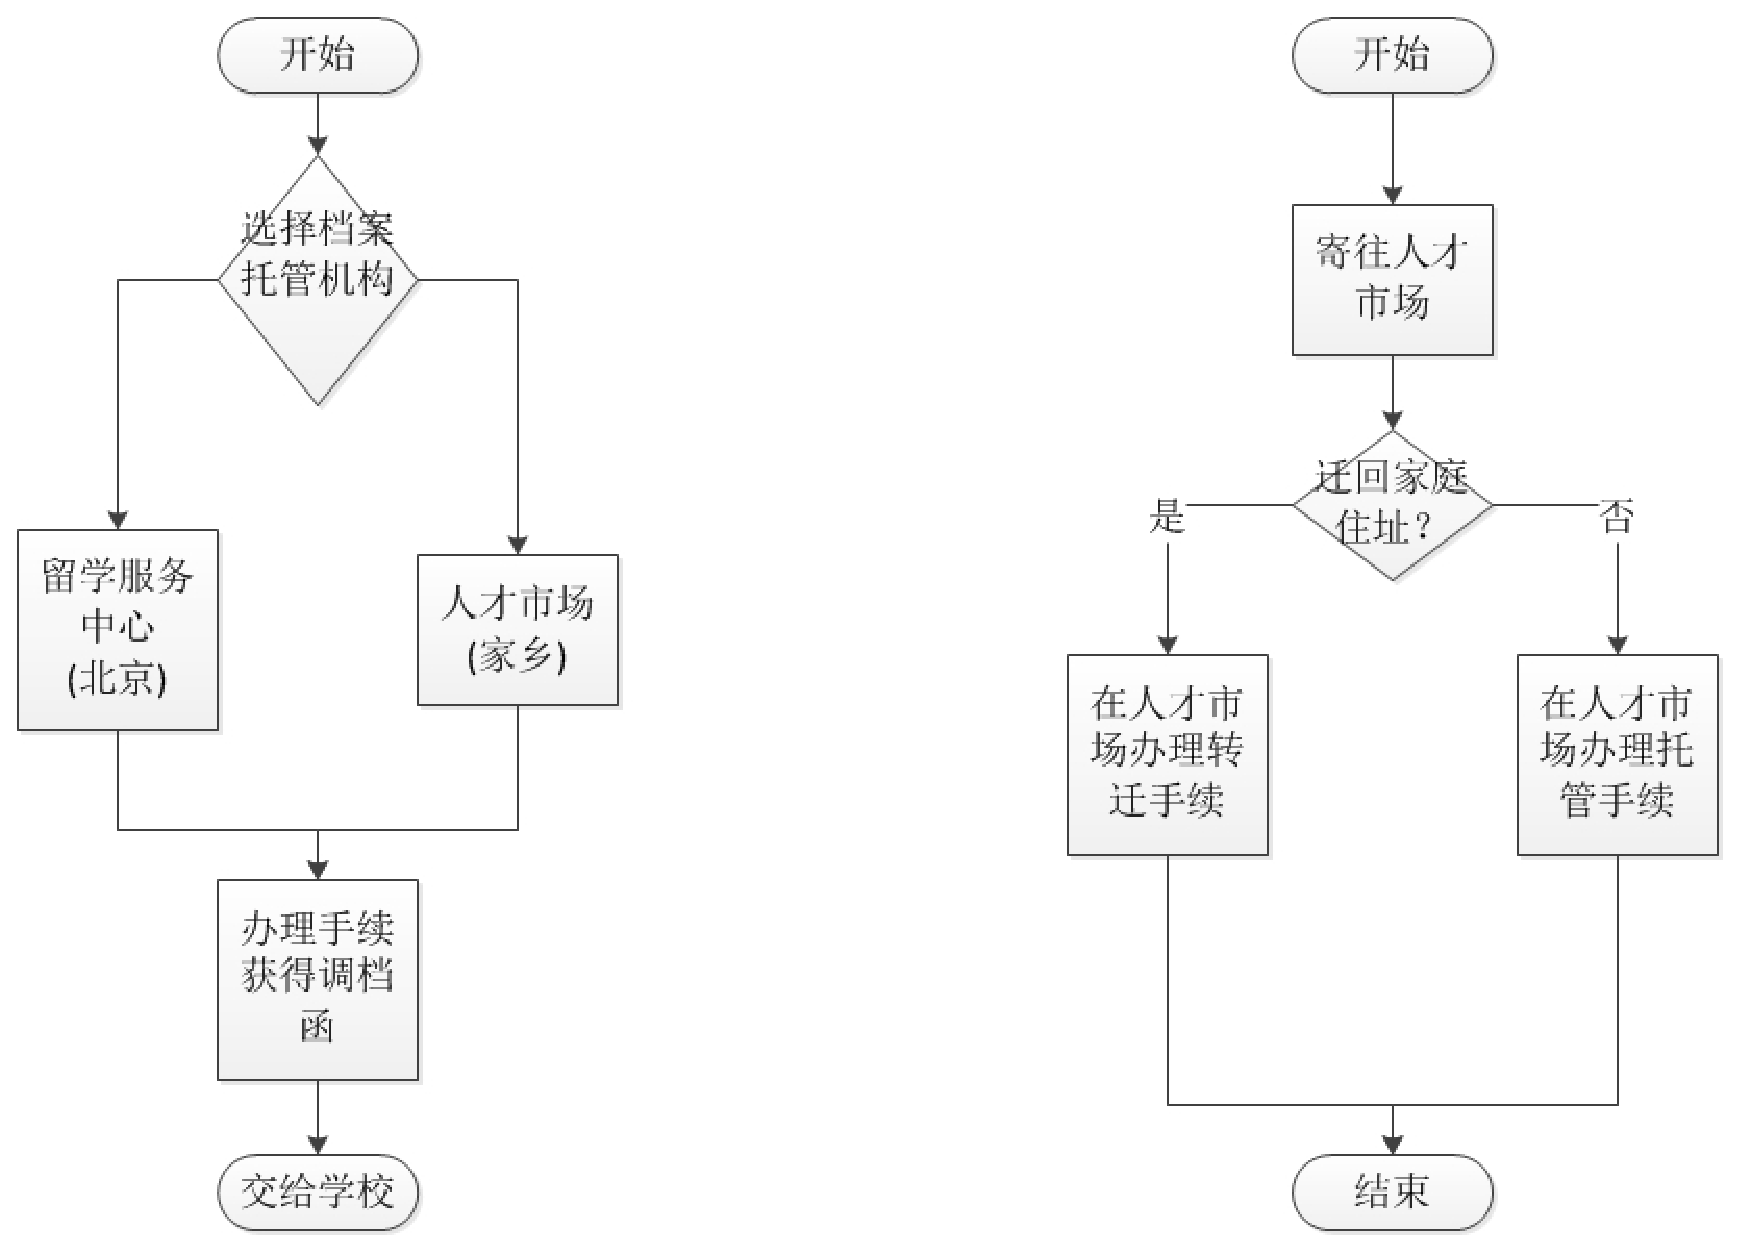
\includegraphics[width=12cm]{4postoffer/hukou.eps}
\end{figure}\par

\chapter{Hello, World!}
\newpage
\section{富士山下}
下面是获得日本早稻田大学IPS项目全奖Offer学长的申请经验。\par
\subsection{基本信息}
名字:庄系舟\par
申请:早稻田大学IPS研究生院Master\par
地点:日本九州岛 福冈县 北九州市 若松区\par
时间:9月;两年制\par
其实是考研没好好准备,考跪了……于是就试着申请了一下IPS。这个offer运气占多,早大给了150w日元/年+免学杂费,给挺多的,于是就去了。\par

\subsection{直接正题}
我知道很多我们院的同学都等着南大和早大的合作项目,但是其实这个项目从去年开始就没有了,所以还得自己申请,在这里要谢谢刘钦老师给的许多帮助,虽然是材料递交deadline的当天才通知的,不过还是很幸运,和日本方面沟通了一下,给了两天延缓期限,让我们完成申请材料。\par
申请没有什么硬性要求,完全是本着宽进严出的方针(不过Master毕业也挺容易的)
入学后先一个学期的通识基础课程教育,学分修满后再选择导师和实验室,和其他学校有所不同。\par

\subsection{申请时间}
申请的窗口期每年有两个,分别是1月和4月。早大的开学可以选择春季或者秋季,像我们大部分人应该是选择秋季的9月开学,要申请的同学请多多关注早大的官网,窗口期会提供申请材料的下载,请大家仔细阅读材料中的guide手册。

\subsection{语言要求}
语言没有硬性的要求,有G、T的分数和日语考试的分数当然最好,没有这些也可以申请IPS。

\subsection{奖学金}
下载申请材料时,请一起下载鼎新奖学金申请表,填写后一起寄出,随后等待电面,电面完半个月后出结果。
如果这个奖学金申请成功了,就没办法再申别的了。

\subsection{必要材料}
\begin{figure}[htbp]
\centering
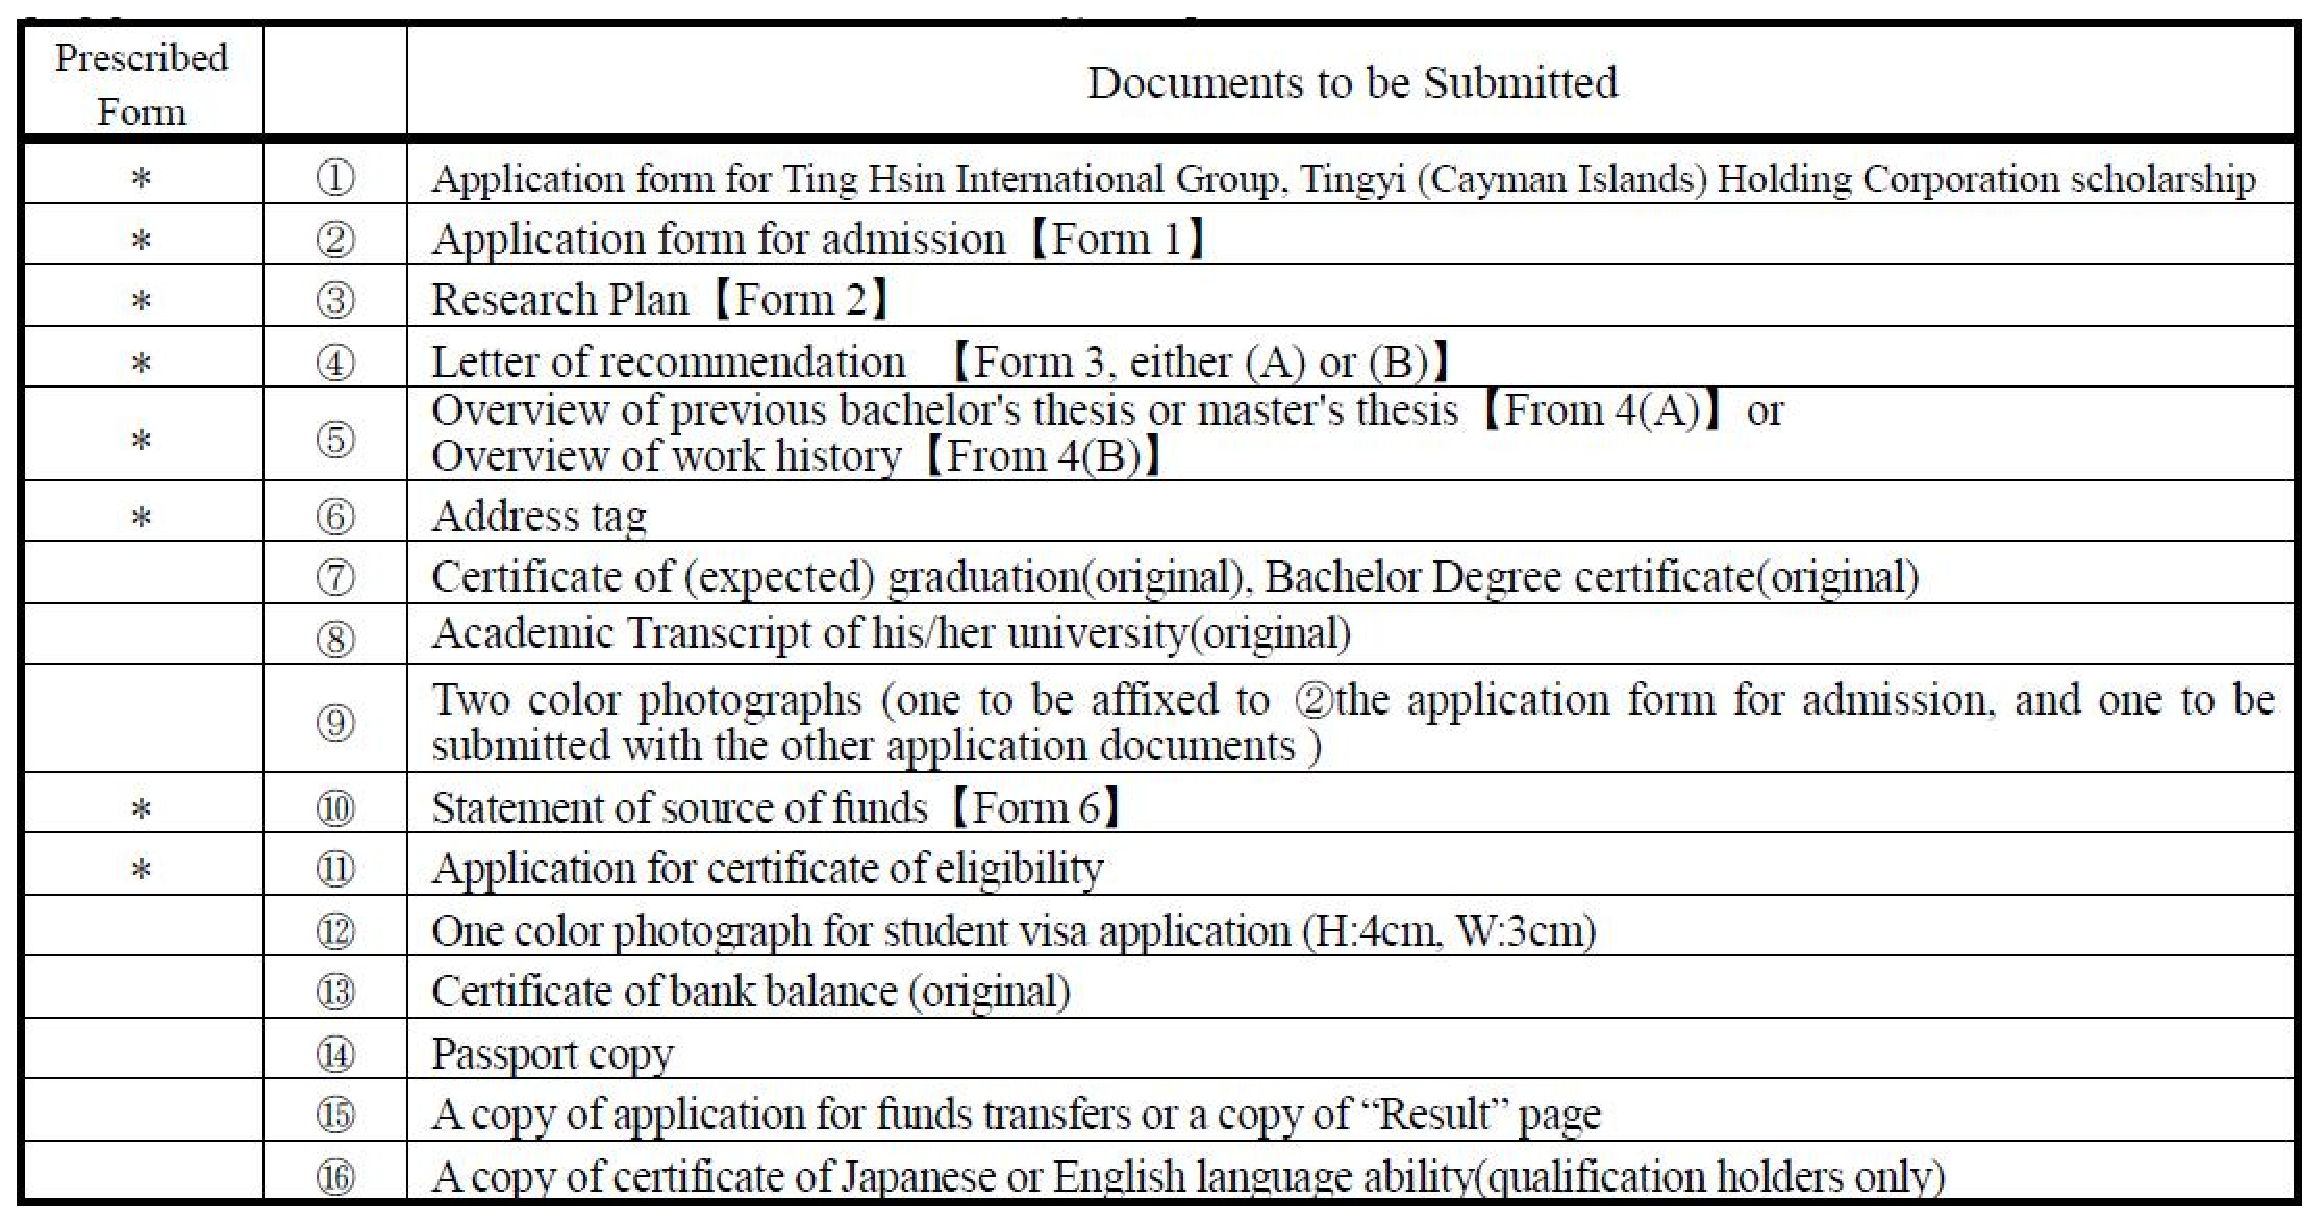
\includegraphics[width=12cm]{5allworld/cite.eps}
\end{figure}\par

其中,打*的是必须按时在deadline之前提交的,如果不申请奖学金,1可以不用提交。没打*的可以等拿到了再提交。\par
其中,1、2、3、4、5、6、10、11,也就是打*的这几项,是从网上下载表格后填写的。\par
第7项,如果还没拿到毕业证书,请到学院找辅导员和教务员开具预期毕业证明(!不是学校教务处的在读证明,请让学院的教务员盖学院的公章)\par
第14项,如果没有护照,最好要在offer寄到之前办好。\par
第15项,申请需要在网上缴纳报名费,缴纳完毕后请保存缴纳成功的网页页面,并打印。\par
注意,一切以官方网站下载的指导手册为准!

\subsection{申请流程}
首先,从官网上下载申请材料:\href{http://www.waseda.jp/ips/english/index.html}{官网地址}。打印之后按要求填写完整后寄出。然后,申请奖学金的请等待电面,电面后等待email通知。最后,耐心等待EMS送来的offer。Offer里有入学流程手册和一些表格,填好个人信息,Student Card, 各种保证书,然后寄去日本,并按照入学流程手册的流程打学费过去。毕业后扫描中英文的毕业证和学位证并email给日本,英文的证件请都去校教务处办理。机票等拿到护照后,知道了入学日期后去买,别买太早的,太早了宿舍不让住,只能自己在日本租房子或者住酒店,学校的宿舍可以在开学典礼前两天入住。

\subsection{学费和住宿}
学费:第一学期77万日元,其后每学期50万日元左右\par
生活费:每月正常花销在5~6万日元左右。(不正常的开销另当别论)\par
住宿:两人间,随机分配,有独立卫浴小厨房,请自带床上用品。费用:每月1.1万日元左右


\section{维多利亚湾}
下面是一位申请到香港科技大学CS硕士的学姐经验。

\subsection{总结}
冒出要去香港读研的念头比较晚,整个准备过程都显得有些仓促,也有很多缺陷,不过好坏都是经验,在此与大家分享。\par

组成木桶的木板长短不一,如果用木桶装水,那所装水的体积主要由最短的木板决定,如果用木桶装熟透的米饭,那么可以利用最长的木板来增大木桶所装米饭的体积。在申请过程中,需要突出自己具有的优势,弥补缺陷。我的GPA较低,80出头的成绩刚好能够满足申请香港各所大学研究生的条件,但在众多竞争者中实在没有多少竞争力。较幸运的是,一年半的科研经验提高了自己的硬件条件。在本科阶段,只要曾参与到科研项目中,即使没有发表论文,都应该在简历或者面试中作出适当介绍。例如,在CV中,可以简要陈列自己曾参与的科研项目,简要描述自己在这些项目中作出的主要贡献,将已发表的论文以标准格式列出,并用粗体突出自己的名字。在PS中,除了突出自己申请该学校、该项目的原因外,也可以委婉地描述自己的优点,向学校陈述为什么评委会应该同意你的申请。申请香港大学MPhil/PhD在申请需要写RP,建议在写RP前与自己研究的课题相关的论文,在RP中可以简要描述自己的研究经历、对具体研究课题的认识(优缺点)、提出可扩展的研究方向。\par

\subsection{申请}
香港的研究生分为MSc与MPhil,MPhil需要跟随导师做项目,申请该项目的成功与否与导师的意向有很大关系,对于没有特别优势的自己来说,套磁是一个必要步骤。在确定想要申请的学校之后,还要选择好的导师,可以通过查看导师的主页、联系导师指导过的学生等多个渠道了解导师的研究方向、个性、指导原则等情况,从而从众多教授中选择出需要套磁的对象。一般情况下,可以同时联系多个学校的多个教授,以节省时间,增大几率,但是不建议同时联系同系的不同教授。在对教授进行了解时,需要知道需要的是什么样的学生,有的教授需要的是勤奋型的学生,有的教授需要的是思维灵活的学生,可以根据具体情况突出自己的优点。如果教授已经肯定了申请者的能力,鼓励申请者申请某个项目,那么申请该项目的成功率就近半了。\par

在选择推荐人时,较幸运的是能够找到与自己想要申请的教授相识的人作为推荐人。因为对于教授来说,了解大多数申请者的途径只是通过阅读CV,PS等文书,教授也会怀疑这些文书的可信度,如果这个时候能够有熟人为自己做出推荐,会增加教授对申请者的信任,提高申请的成功几率。\par

无论是CV,PS,RP还是RL,在提交之前都需要从文书组织结构与语言语法两个方面进行重复修改。这个阶段可可以找专业培训机构,或者在国外的朋友帮忙修改。这两个方法我都尝试过,在修改文书之初,我先找了南京某培训机构的一名老师,但是修改后觉得效果欠佳。后来请了一些有申请经历的朋友帮忙,重复修改了很多次,才敢提交申请文书。个人感受,如果能够找到那些了解自己并已经熟悉国外思维模式的朋友帮忙,能够为申请者节省很多精力。当然,申请者自己也需要一遍遍地对文书组织结构进行修改,一是因为申请者应该充分熟悉自己的文书内容,二是最了解申请者经历的人是申请者自己。

\chapter{随想集}
\pagebreak
\section{李皓寰 UCSD}
我的出国申请也算告一段落了, 回想申请时的各种经历, 教训, 感想, 发现有很多值得分享的地方, 这里写出来当时为将来申请的学弟学妹指指路吧。\par

       首先说一下我的申请结果吗, 我全申的MS: 
\begin{itemize}
\item        AD: Upenn, Wisc, UC-Davis, UCSD(Accept)
\item        Rej: PSU, UIUC, UT-Austin, UCSB
\item       Pending: Brown, UNC, Umich, Rice, UCI, TAMU
\end{itemize}


\subsection{为什么要出国?}

出国是一项重要的决定, 你要么得奉献出五六年的青春, 要么就得付出高额的花费。出国的原因可以有很多, 西方的教育, 异国的风情, 不一样的学术科研环境, 等等。 我当初选择出国,纯粹是一种随波逐流。 记得是大二寒假的高中同学聚会, 很多人在讨论GRE,TOEFL之类的东西,听着不明觉厉,加上自己当时成绩也不错, 英语基础也算扎实, 于是抱着好奇的心态萌生了出国的想法。但是当我掂量了一下红宝书的厚度后,突然就心里虚了,有种还没迈出一步就栽了个跟头的感觉。当时寒假买下红宝书时计划在接下来的大二下学期把它啃完, 而实际上直到学期结束,我才啃完三分之一。\par

这个时候我内心里出国的想法已经动摇了,单词背不下来,出国花费又那么高,读博又那么苦那么久,再加上我们这个专业不管是读研还是工作都可以有很可观的收入,何必要为难自己去经历出国申请的那些苦呢? 我一度把背单词的计划搁置了两三个月,直到有一天我看到了肖复兴写的一篇散文"年轻时就应该去远方”。我现在都觉得有些不可思议,但是回忆起来确实就是这篇文章让我的想法产生了180度大转弯。 这篇文章的一些观点确实是发人深思的,漂泊他乡,是一种苦,一种累,但更是一种挑战,一种宝贵的人生经历。 出国留学为了什么? 这个问题事实上是把出国留学手段化了。在我看来,出国留学本身也可以是一种目的,漂泊国外的种种经历和考验所带来的内在价值,远比一个海外文凭所带来的经济和就业效益这样的外在价值大得多。

\subsection{Phd?Professional MS?Acadmic MS?}

在决定出国之后, 接下来的就是学位选择的问题。 学位总体上两种: Phd和MS, 但是计算机专业(不知道其他专业有没有)里面MS又可以分为Professional MS和Academic MS. 前者适合将来想出去工作的, 主要就是上课做作业。 后者适合将来转Phd的, 除了上课外可能还会做研究, 当然也有机会拿RA。\par

鉴于读MS高额的花费, 我曾经也有个读Phd的想法,我也花了不少时间去了解Phd这个学位。在我看来,与其说Phd是一种学位,倒不如说它是一种职业。学生的本职工作就是上课考试做作业,完成这三项任务就算OK了。但是Phd不是,Phd虽然也需要上课,但这已经不是他们的重心。他们的主要工作是做研究,看论文,写报告。Phd免学费且有钱这确实很吸引人,但这实际上都是通过辛苦的搬砖换来的。虽然很多学校都有全奖(Fellowship)这种东西,但不是所有Phd都拿得到,即便能拿到,最多也就维持一年。大部分Phd都要依靠研究项目的Funding养活自己。在我心目中,Phd是一个神圣而严肃的东西,不能随随便便说你想读就去读。Phd是一群某个领域的狂热爱好者,它们愿意奉献自己的青春年华,甚至一辈子给这个领域的研究。科研就是他们的爱好,一连串的挑战带给他们的不是畏惧而是兴奋。虽然他们面对着这个世界上最强的智商考验,但是他们不求太大的经济回报,因为征服这一连串考验,就是对他们最好的回报。我觉得如果不满足这些特点,最好不要尝试去读Phd。也许我把Phd有些妖魔化了,但是我觉得妖魔化点也好,因为Phd是一个求精不求多的东西。\par

我很早就断去读Phd的念头,但是我在Professional MS和Academic MS之间踌躇了很长一阵子。这两种硕士可以类比为国内的专硕和学硕。美国的MS大部分都是前者,我所知道的的提供后者的学校有UIUC, Wisc, Rice, UNC。虽然我将来是想工作的,但是我一开始的想法是读Academic MS,  因为我害怕Professional MS的课会像大软院的课一样。我当时认为Academic MS可以在课余时间可以跟教授做项目,这样既上了课又捞了研究经历,一举两得。但是我发现这种如意算盘在课业繁重的美国大学里是行不通的。我有一个同学在RPI读的本科,他常常会做作业做到3点睡觉,如果你常常逛一些出国论坛,会发现大多数留学生都常常会有一波due赶得死去火来的经历。Academic MS实际上是一种Phd后备军,他的生活方式是与Phd比较类似。如果不想Phd,最好还是不要选择Academic MS的。我申请的时候申了3个Academic MS,申完实际上就有些后悔了。\par

总之,美国学校里不管是上课还是做研究,都是很专业的,最好不要有两者兼得的想法,你只拥有做好一件事的时间和精力。在中国可以看到不少教授旗下挂着一堆项目,这在美国是不现实的。

\subsection{GRE TOEFL}

 GT在申请中重要性可以用“鸡肋”这个词来形容: 你说它不重要,但低GT有时就会卡死你; 你说它重要,但光靠GT又很难让你脱颖而出。在这个GT通胀的时代,G1350+4.0,T105(22)已经是个很平庸的水准了,我的GT甚至还不及平庸。但是如果能有个G1500+ T110+ 那就另当别论。\par

我准备GT的过程是很不专业的,首先是没上过新东方,其次准备时间也较短。我考GRE的经历还是算幸运,当时扭转心态决定出国闯荡的时候,距考试已经只有不到两个月的时间了。那时红宝书第一遍都没看完,看过的都忘得差不多了,这个时候显然常规的准备方法已经行不通,所以我只能尝试投机取巧的办法。首先我放弃了红宝书转而看高频词汇,当时我看的那本书是新东方的”高频词汇句子填空“,好像有一本类似的书叫”要你命3000“,在时间不足的情况下,看高频词汇也算得上一种合理的方法吧。填空觉得完全拼的是词汇量,5个选项全能看懂那这个题基本拿下了,要是一个都看不懂那就只能试人品了。填空这部分的实力是需要长时间积累才能获得的,如果时间不够,建议不要在这上面耗太久。对于阅读,我当时的准备材料就是一个网上下的一组练习题,名字已经不记得了。我当时就是每天练两篇。我想强调的是阅读一定要上机练,这样可以方便你适应机考的环境。对于作文,我就花的时间就更少了,我在考前两个星期才开始学写Argument,考前3天才开始练习Issue, 要不是考试的时候Issue题目正好是我之前构思过的,恐怕我的作文就完全跪了。 GRE作文的特点就是强调结构和逻辑,观点鲜明,逻辑通顺放第一位,语句优美流畅等等都在其次。它考察的是逻辑分析能力而非语言能力。我最后GRE考了个154 167 4.0, 不到两个月内能游这个成果我已经很欣慰了。\par

至于TOEFL, 我觉得最好的练习材料就是官方指南和TPO。如果你不是一个很有口才的人,那口语一定要尽早开始练,否则到考场上时会发现自己的舌头像打了结一样。练口语也不仅仅是光说说就可以的,需要录下来,自己听听然后给别人听听,看有什么地方可以改进。给别人听是很必要的,当时我准备二战的时候狂练口语,但是却忘了给别人听,结果考的时候自我感觉良好,出分发现还只有20,复议才给了22.\par

\subsection{选校}

当你考好GT, 弄好成绩单之后, 就可以开始选校了,当然也可以在选校的同时准备PS和CV。选校也是一件很麻烦的事,我当时选校的时候完全没有头绪,于是就去一亩三分地论坛发了一个定位帖。这里顺便说一下,一亩三分地是一个很好的留学交流社区,它有很好的板块分类,并且这里面几乎没有灌水帖,这也是我最喜欢的一点。在这上面有很多人都发过定位帖,一般也都会有人回复。回复你的不一定是牛人,也许他也是个学校的小白,但是当我看到很多人都在和我同行,向着同一个目标奋斗时,我感到很欣慰。一群人一起探索未知总比一个人探索未知好,虽然交流会浪费一些时间,但至少你不会觉得孤独,这不是最有效的方式,但却是最开心的方式。以我看过这么多定位帖的检验,发现选校的档次大抵是和GPA成正比的,所以在大学前三年一定要好好上课。一般人选校的时候都会按照US News专排分三个档: 冲刺档, 主申档, 保底档。 当然不同人也会有不同的地区偏好, 想过得舒服的一般都会往加州跑, 将来想去银行的一般会去东海岸, 喜欢到处逛的一般会选择LA, NY这样的大城市, 喜欢田园风景想远离城市喧嚣的一般都去德州大农村。 我觉得选校这个事情不必太纠结,想申就申, 等到拿了AD之后再纠结也不迟。 

\subsection{PS, CV}

PS和CV是留学文书中最重要的两项, 也会最让人头疼的两项。PS因为文字更多, 所以相对更难。这里我先分享写PS, CV的一亩三分地精华帖: PS就是最好的套磁,如何用CV打开申请之门。这两个帖来自于同一个作者, 其中很多观点都很有指导意义。作者在我看来也是一个非常牛B的人物,可以看一下他的申请历程,当看到他做过的项目时,我就已经完全吓尿了。 我觉得PS要达到3个特点: 真实性, 独特性和简洁性。真实性无用多说, 独特性是很重要的, 如果你没有亮瞎眼的硬件,那就得靠独特的PS来吸引commitee的眼球。好的PS至少得要个独特的开头,我不提倡用" My name is.. ", "I am .." 这样的句子来起头,如果让committee看到这样的开头, 他们很可能就会认为又是一篇平庸的PS然后直接将后文一扫而过了。简洁性也很重要, PS一般不要超过两页, 冗长的PS和平庸的PS一样让人反感。写PS是一个痛苦的过程, 要做好改的准备,我写的PS至少大改了4次,小改就数不清了。PS最好给学长或老师看一下, 他们以旁观者的视角很可能提出一些很有用的意见。CV可以看做是一个大学经历的精炼总结,你可以写上自己做过的项目,参与过的实习,或者其他非学术经历,总之就是起一个对PS的补充作用,让委员会更全面地了解你,所以CV和PS尽量不要有重复的东西。CV在内容上也可以独特一点,但是格式上一定要专业,网上有很多CV的模板,都可以照搬。\par

留学文书中还有一项是推荐信。有一句话是: 中国人的推荐信只要不是牛推,就都一样。我一个学长还告诉过我一句话: 在南大,除了周志华的推荐信,都不是牛推(当然仅限CS专业)。 推荐信对于国外的学生可能有些分量,但是对于中国学生来说,已经可以用鸡肋来形容了。据说在美国,如果只是课程教师,推荐信不会超过5句话,所以老外一看到中国学生的推荐信就知道是学生自己写的。 这里我提个醒,如果要找老师写推荐信,一定早点说,有些很忙的老师你跟他说得晚,他就不高兴帮你写了,我就遇到了这个情况。\par

\subsection{申请焦虑症}

申请的时候都会有些焦虑,特别是当周围保研工作的同学都早早确定下来,各种happy,而自己却在为申请弄得焦头烂额的时候。这个时候人会心里发虚,填网申表格的时候总会检查一遍又一遍。看到论坛上的各种牛人,便会怀疑自己的实力,心想自己是不是定位过高。这种焦虑是申请时必定要经历的一个过程,我也经历过,也被它折磨过。对付焦虑的最好方法就是心无旁骛,该怎么申就怎么申,尽早申完。申完之后就大可以把申请的事丢到一边,干点别的事,静等offer/AD。愁是没有用的,没有offer/AD是愁来的。虽然网申和文书准备是一个重要的过程,但它并不能起到决定性的作用。申请时的竞争力大部分是由前三年的努力决定的,在开始准备网申的时候,你的申请竞争力你已经基本定型了。那些文书起到的作用只是让你的能力特点更好地表现出来。 所以申请到了这个阶段时,你完全淡定下来。\par

 以上都是本人关于出国申请的一些观点看法,不求正确,但求有所用。出国留学是一个很好的人生经历,如果有这个想法,不要轻言放弃。最后引用电影《当幸福来敲门》中的一句台词: "You have a dream, you gotto protect it."    
\pagebreak
\section{罗钊燚}
时间仓促,匆匆写下此总结,文笔略差,多多包涵。水平有限,学神请绕道。\par

本人南京大学软件学院09级本科生一枚,一共申了11所学校,其中美国8所,加拿大1所,英国2所。全部申的CS Master。\par
\begin{itemize}
\item Accepted: Waterloo CS的Master,32000加元一年(包括RA,TA)。做自动化测试、导师不错。
\item Decline:Cambridge,奖学金是offer发了后再办的(英国的奖学金不一定是学校出钱的,很多机构funding那种),decline之前没拿到奖学金。
\item Rej:Purdue、Yale、Princeton,Oxford
\item 其他:CMU CS\&EECE, Michigan, UCLA,Columbia
\end{itemize}\par
条件:GPA 4.2,有出国交流经历,会议paper一篇(IPDPS,B类偏上)。雅思7.5(美国大部分学校还是认可雅思的,一般要求7分),GRE 157+169+3.5\\(2013年1月5号),153+168+3.5(2012年11月25号) \par
关于GPA、上课:平时学习比较随意,考试压力不大,导致成绩普遍不高(大多80出头,大概有10门70多的),但学到好玩的东西就很来劲,几门核心课程成绩不错(数据结构96,机组原理96,操作系统93,网络92,编译原理89,算法88)。总体来说GPA偏低,成绩分布方差很大。大三出于装逼的目的坚持不重修、不注销、不为学分绩折腰,直接导致与不面试的美国MS program基本无缘,现在想来挺后悔。我的经验是:能考好的课程尽量一次性考好,失误了的如果在80分以下最好重修掉。\par 
\subsection{经历}
下面按我最擅长的方式(记流水账)写下经历吧:\par

大二暑假参加了为期2个月的交流项目(Pembroke-King’s Summer Program, Cambridge),选修3门课程,另外可以选择tutorship,名额有限,有Cambridge导师一对一指导做2个月的研究项目。在此隆重推荐,在各方面都能学到非常多的东西,去了绝对不会后悔(在此不详说了)。申请过程和国外Master申请的流程差不多,要求成绩单、一封推荐信、雅思7分、一份written sample等,review 3周后给答复。2个月的费用约为学费2000磅+生活费1500~2000磅,tutor额外500磅(有cover学费的奖学金,名额很少,而且要提前申)。\par

 

大三下学期,从2012年1月到10月,大部分时间在做研究,花了很大精力(不是创新项目,就是普通的跟着老师做那种),最后paper发在一个国际会议上(IPDPS,B类偏上)。经验:科研经历最重要的不是经历也不是发paper,而是提升自己的学术素养。面试的结果通常是决定性的,压倒其他一切经历、GPA、获奖证书等,而面试考察的就是学术素养。可以认为,在有面试环节的申请中(英国的牛剑、加拿大的学校以及美国的PhD),其他经历仅仅为了得到面试机会而已。\par

 
\subsection{申请}
下面是申请(我着重说一下加拿大和英国的,美国的悲剧了就不说了):\par

paper写完就是10月初了,时间已经很紧了。我花了1个月时间背GRE单词(平均每天7小时),背完后11月初颓废了10来天宅宿舍玩游戏,然后2周准备GRE、刷题(作文基本放弃),11月25号考G,接下来3天写申请文书、弄推荐、提交了5个学校的申请(马上申请就截止了),然后开始了长达几个月的颓废。期间,12月中旬申了剩下的6所学校(基本也是马上申请就截止的);套过CMU的一个教授,跟我一样的做云计算,我跟他说我看过他的paper,很有兴趣(实话),然后把我做的paper发给他,结果杳无音讯;12月12号Cambridge电话面试,面试内容是先自我介绍,东拉西扯,然后对一篇提前发给你的paper做分析(所谓的学术素养)。面试发挥得不够完美,本来感觉达不到Cambridge这种高端学校的标准,但1月17号还是收到了condition offer(莫名其妙)。12月30号Oxford一面(或者叫笔试吧),用邮件发一些算法问题,作答。回答自我感觉很满意。1月11号Waterloo的一个教授发来邮件,说看了我的简历不错想邀我面试(传说中的被磁套?),然后我跟我们院里的老师打听了下这个老师,据说挺牛。面试的电话打了大概半个小时,仍然是先介绍下我大学的学习情况(他会在他感兴趣的地方打断我问我问题),然后东扯西扯,扯得差不多了我说我看过他的paper(面试前几天看的),他说that’s great! 然后开始扯paper的内容(发挥所谓的学术素养的时候又到了),面试结束时他说It’s very promising, I am not decided yet but I will definitely take this seriously。然后我们通过电子邮件keep in touch,我继续看他的paper,说说自己的想法,也会回答他问一些问题。大概过招4、5回合后他就从了,决定招我。2月6号offer正式发下来了,2月10来号我accept了waterloo的offer,decline了Cambridge。2月底Oxford二面,问的是马科夫链的不可归约性、极限概率解唯一的条件(因为我发的paper里用到了马科夫链,他以为我比较了解)。结果因为已经从了waterloo的offer了,没好好准备,知识也早忘了,面得惨不忍睹(学术素养不够高啊)。不出意外面试后的第二天就受到rej了。后来我把这些基础知识再狠狠地学习了一遍。

 
\subsection{经验}
下面归纳几点重要的经验:\par

GPA别太轻视,目标是每门80分以上。80分一下的最好重修,但尽量一次性就搞定,因为重修也是要耗时间精力的。\par
出国交流重要的不是经历,而是提升综合素质。。\par
不要好高骛远。研究刚起步就把top conference如数家珍似的了解个通透是没有用的,就像没钱买一个轮胎还整天把各种豪车挂在嘴边一样可笑。脚踏实地地一心做学术才是硬道理,肚子里有货了再来了解这些也不迟。\par
搞研究重要的不是经历,也不是发paper,而是提升学术素养,面试时也用得着。\par
心态要端正,国外不是天堂,不是dream,结果怎样都无所谓。反正我是抱着收齐拒信回家种田(码农也是农)的觉悟做的申请\par

最后,我自认为对大局观把握得比较好,而不擅长各种细节(或技巧)处理吧,如文书怎么写,申请怎么弄,套磁怎么搞,单词怎么背等等没有有用的经验可以分享给大家,自己也没觉得这些做得有多出色。另外,经历较奇葩,大家挑着顺眼的看就行,希望能对各位的申请有所帮助。祝大家offer多多!
\pagebreak
\section{徐达博}
背景:
\begin{itemize}
\item Revised GRE:Q170, V155, AW3.0
\item TOEFL:105(23)
\item GPA:85+
\end{itemize}
\par
申请结果:
\begin{itemize}
\item Admission:U Az, PSU, MISM@CMU, UCD, UCSD, TAMU, USC
\item Rejection:U Wisconsin-Madison, UPenn, Berkeley, Columbia
\end{itemize}
\par

\subsection{我的背景}
申请中最出彩的地方是什么?这个是一个学弟问我的问题。说实话我也不知道是哪一点让审我材料的教授就砰然心动了。但是对于我自己感觉来说,申请当中经历最丰富的,帮助最大的,当属在UC Davis的9-12月吧。\par

在戴村我最后三门课程拿到了3.9/4.0的GPA,虽然UCD的课很水,大家分数都很高,但是表面上看过去,还是很让人赏心悦目的成绩单。此外感谢和我一起考试的韩国友人、印度友人和南美友人的口音,我拿到了105的托福分数。不过每次T我都没有认真准备,基本是考前准备模板的半裸考状态,所以最后105真的都是靠运气,还希望大家吸取我的前车之鉴,早点考GT,早点刷GT。

\subsection{文书准备的一些建议}
文书包括了PS和CV两个,PS主要阐述Why 这个学科, why 俺们学校, why 俺们系这三个问题,当然不能直白地回答,要艺术性和创造性地结合自身经历,让看材料的人觉得你天生就是为他们这个项目生的。一定要让Native Speaker帮你改语法,让同专业的学长学姐帮你把握PS结构。

\subsection{关于MIS}
实际上,我并不鼓励大家都不申请CS的方向转而申请MIS,因为对于中国人来说申请MIS和CS最后还是殊途同归要去做Tech,而往往CS在就业这方面占了巨大的优势。W大总结的很好,CS人多机会多,MIS人少机会也就少一些。\par

那么我为什么还要申请MIS呢?因为个人非常喜欢CMU这个项目,觉得他就是教给我想学的东西,此外可以旁听些感兴趣的CS课程。反观CS,深知自己会给大神们当炮灰,所以就没有再念CS了。\par

对于CS related转申MIS的同学,我建议你们在申请MIS的同时,千万不要忘记去申请CS的学校!和CS相比MIS的好处就是Broaden your horizon, 让你除了技术还有更多的相关知识,这和软工的知识有异曲同工之处,就是你要有了丰富的工作经验之后回去看,才能对这些知识有深刻的体会。那么CS的好处就是你继续相关专业的学习,有很多时间可以准备面试,一般的CS项目是两年,有充分的就业时间准备。所以归结起来,技术是你的武器,无论什么方向,都只是一个平台而已,\textbf{机会要自己争取}。

\subsection{一些补充}
我非常希望软院出国的人越来越多。其次,通过建立考试互助小组的经验让我相信同学之间的不应该只有竞争,还应当有合作和共享。但是因为一个学校录取很多NJU SEer的可能性很低,所以基本上某学校如果我们院申请的人多,那么我们还是要在内部选出一个来,这样的情况下大神拿到AD的概率就是非常大的。所以在申请过程中的互相通气蛮重要的。

我的邮箱:dudnju+applyforus@gmail.com

\pagebreak
\section{姚佳玮}

背景:
\begin{itemize}
\item GPA: SE@NJU, 90.0, 2/185
\item GRE: 158+169+4
\item TOEFL: 113 (23s)
\item Paper: 学校创新项目,国内水文一篇
\end{itemize}
\par
申请结果(CS MS):
\begin{itemize}
\item AD: Stanford, UTAustin, UMich, UCSD, UPenn, Brown, UCI
\item Rej: UCB, UIUC, Dartmouth
\item Withdraw: UCD
\end{itemize}
\par
\subsection{关于定位和选校}

MS的申请没PhD那么有玄机,基本是拼硬件。定位全看背景,学校、GPA、排名、GT、科研等都是要考虑的因素,一亩三分地W大有免费定位,认真填表即可,他会给你一个大致的方向,参考价值较高。偷懒一点可从往年的申请者中找和自己背景差不多的参考,这在没有太多精力了解每个学校的情况下很有用(说说而已啦,多花点时间啊少年)。\par

选校的话记得找自己顺眼的,不要最后给了你AD都不想去。通过人家主页多了解下,不明白的地方尽情问小蜜,不要钱的哦。数量10-20左右,记得拉开档次。还有不必迷信“申请的人太多肯定当炮灰”、“这个学校不收我们学校的人”这种说法,出国的越来越多,每个学校申请人数增加是肯定的,另外每个学校给AD的标准都不同,不要自己给自己限制。\par

申请材料和文书的具体指导可以参考我的这个\href{http://d.pr/f/UgYx}{slides} 。

\subsection{关于申请}

大家可以多关注下rolling的学校(UPenn,UTD,NEU等),早提交早出结果,方便结束三无状态。比如UPenn有三个cycle,第一个deadline在11月15号,11月底就出结果。如果拿到AD就是吃定心丸了,就算拿到Rej也可以拿来校准你的定位。\par

排名靠前学校的deadline扎堆都在12月15日,由于申请过程中不可控的因素太多,大家就不要玩火踩deadline了,会吃不好睡不香(比如像我一样T\_T)。还有到申请末期免不了手熟就不认真看instruction,如果这所学校不是可有可无,还是认真填吧,不要出岔子了(比如我申UCD的时候手一抖把出生地填成Central Repub of Africa)。\par

网申完毕并不代表申请就完了,勤查状态,要等材料、GT成绩都到了才能放心。之后就等结果吧。

\subsection{关于申请结果}

就今年的经验看,CS MS集中在三月中下旬出结果(PhD好像一月就开始陆陆续续出了)。我除了UPenn的AD是11月底收到的,之后一个AD是2月底到的,最晚的一个是4月6号刚收到的。更有同学5、6月还收到AD,所以就算连续Rej也别太灰心,战线很长呢。\par

MS项目的话,大多数学校都是遵守4/15的,就是学校不能强制学生在4月15日之前答复,即使accept了也可以反悔。所以4/15之前,如果你有多个AD,不要提前纠结,如果来了个dream school之前的纠结就白费了是吧?当然一般情况是,有了几个可以take seriously的AD,这时候除了纠结,记得把来了AD也不会去的学校给withdraw掉,不仅对其他申请者有利,还能攒RP。同理,如果你最终决定accept一所学校,其他给了AD的学校也decline掉。

\subsection{关于Stanford}
之所以Stanford收了我,我觉得主要有三点原因:\par
\begin{enumerate}
\item 硬件足够。对于MIT、Stanford这种学校,我们学校肯定不如清北有优势(人家排名20、30的都非常有竞争力),所以top的GPA和GT成绩是不被刷掉的保障。这里说一下,S的T要求113,这个和布朗的105一样,其实不卡,不过入学后可能要上英语课。
\item 有分量的推荐信。给S的三封推荐信各自来自课程老师、科研导师和实习老板,内容都比较strong,从学习、科研和工作三个方面证明我的能力,算是比较让人信服吧。
\item 有亮点的文书。S的SOP我是单独写的,整篇以startup为主线,讲创业的重要性,以及我自己立志创业和参与创业的经历,算是和Stanford代表的硅谷创业文化比较match。加上之前是互联网上市公司高管、现在在创业的老板的推荐信,也增加了说服力。
\end{enumerate}

\subsection{一些建议}

出国申请总体上来说是一场拉锯战,希望大家能尽早、认真准备。大一大二好好刷GPA,大二大三好好考GT,大三大四扎实文书和申请。知己知彼,百战不殆,最了解你的就是你自己,所以我不建议把一切都委托给中介;有时间就多了解了解目标学校的招生特点。多上一亩三分地,多和一起申请的同学交流,stay tuned,不要孤军奋战。\par

另外,出国交流是提升背景的有效手段。身边无数的例子表明,去过A校交流拿A校保底的可能性就很大,就算不能保底,能拿到老外的推荐信也更有分量。\par

人人上有一个我申请的总结,有兴趣的戳\href{http://blog.renren.com/blog/282030513/900352093}{这里}。

祝大家都能申请到理想的学校。我的邮箱:kavinyao@gmail.com
\pagebreak
\section{叶韵致}
背景:
\begin{itemize}
\item GPA: 86/100
\item TOEFL: 103 (R29+L28+W27+S19)
\item 无研究、无牛推
\item 实习:外企实习六个月(eBay水实习)
\end{itemize}\par
申请结果:
\begin{itemize}
\item AD: Columbia, Rice, UCI, Stony Brook, TAMU, UC-Boulder, NEU
\item Rej: Yale, Upenn, UCLA, UCSD, UMASS, UFL, Gatech, Dartmouth, Brown
\item Pending: USC
\end{itemize}
最后去了Columbia。\par
一句话概况起来,这次申请不算成功,也不算失败吧。最终去的学校也算是比较满意了。
下面详细介绍一下我的申请总结和教训吧。
\subsection{关于GRE/TOEFL}
就我的申请结果而言,我觉得GRE/TOEFL过线就行了。尤其是GRE,感觉大部分学校都不怎么重视GRE的成绩,一般320是一条线,过了320的话GRE就不会拖你后腿了,不过超过330的GRE是一个亮点,尤其是对个别比较看重GRE成绩单学校(比如yale,录取的人都有超高的GRE成绩)。TOEFL过100,应该算是硬性要求吧,虽然很多学校的招生网站上说,他们要求的托福底线是85,87什么的,其实他们实际录取的情况都比这个要高很多,一般观点是100分是一条线。其实过100并不难,屌丝如我的英语四级没上550,六级没上500的学渣,努努力还是能上100的。\par
至于如何准备GRE和TOEFL考试,我就不多说了,一者,我两项成绩平平,并没有什么比较牛逼的应试经验,二者,网上很多牛人分享的经验,一搜一大把,而且我觉得他们都说得挺好的,我就不重复了。不过GRE和TOEFL的确是需要花时间和经历的,当你过了这两道坎,申请也成功了一半了。
\subsection{关于GPA}
GPA绝对是申请里面的重头戏。除开各项软实力,单看这几项硬实力,GPA远大于TOEFL、GRE。GPA的重要性自是不容忽视的,平均分85是一条线,越往上走优势越大,到了90的平均分是具有很强的竞争力的。所有课,不管是选修课还是必修课,都要一个劲往高了考,因为申请的时候,对方学校不会管你是不是选修课,统统加在一起算你的GPA,所以不要因为是选修课就无所谓。当然水课和好课的权衡要靠你自己了,水课容易得高分,但是学不到什么东西;好课可能意味着较低的成绩(牛人请无视),但是能够学到实实在在的东西。 所有课尽量保持在80分以上,没上80的话就重修吧(如果是毛概,马哲什么的,还是算了,随他吧)。不过重修还是要量力而行,自己把握课程压力,不然得不偿失。
\subsection{文书准备}
软实力其实是我很想在这个总结里面讲的内容,因为我的申请就差在了这个方面上。软实力包括很多,科研,交流经历,实习经历,我觉得推荐信也算是软实力。\par

科研,直接衡量标准是论文。论文虽然对于PHD申请者来说更为重要,但是2013FALL的经验告诉我,有了论文,Master申请也会平步青云。因为在申请的时候你会发现,你的竞争者们很多手握一两篇论文,和你一起抢master的坑,所以可以搞搞研究还是尽量参与到研究中去,一方面可以深度了解某一个具体的领域,一方面有机会发论文,再一方面还有可能套到牛推。\par

交换经历也很重要的!有交换经历的同学,一方面可以拿到外国教授的推荐信,另一方面可以获得国外学校的成绩单。对于你要申请的学校而言,他们并不十分了解中国的学校的情况,你的成绩好坏对于他们来说并没有直观的认识,如果你有国外大学的成绩单,这样他们对你的学习能力就有数了。而且国外本科拿个很高的GPA对于你们来说应该不太难。\par

抛开其他的方面不说,功力地分析实习经历,如果你是去MRSA或者中科院什么的去实习的话应该会加分不少,其他地方的实习经历对于出国申请帮助不大。所以,如果功利一点,能去那两个地方就去,去不了可以留下来跟着学校老师做研究(当然,去清华北大做研究也可以,还有海外研究也是一个非常不错的选择)。不功利的讲,去创业公司实习收获最大,当然也最辛苦。\par

下面是我想介绍的整个申请过程中了解到的一些学校的信息,希望这些信息对以后的学弟学妹有帮助吧。

\subsection{学校信息}
\textbf{UCLA}\par
综合排名:24 专业排名:14 申请难度:***** \par

UCLA是曾经的dream school啊。但是看了他给的AD的申请者的背景,顿时就萎了。各种论文哥,各种高GPA,申请难度和Stanford有的一拼。当然UCLA如此傲娇也是有他傲娇的资本的。地处加州洛杉矶,地理位置的优势为他加分不少。加州对于CS专业来说毋庸置疑是块风水宝地。各个IT巨擘还有数不胜数的创业小公司,为加州的CS行业推波助澜,形成了一片祥和的景致。因此这也为加州系列的各大学提供了非常强劲的竞争资本。\par

当然,如果只是地理位置好,UCLA还不能如此傲娇,最主要的还是要依仗他的计算机实力,UCLA的计算机科学实力不容小觑,从排名就可见一斑,尤其是他的AI和ML方向,非常之强(AI和ML也是现在很火的方向之二)。\par

所以,要拿到UCLA的AD,并不容这么容易,发几篇论文,搞高GPA是很有必要的。\par

\textbf{UMASS}\par
综合排名:97 专业排名:20 申请难度:**** \par

UMASS 招master很少,基本只招博士。Master招过去基本也是搞研究,而且很有可能有奖。不过招人很少很少,它的AI特别强,貌似排名前十。UMASS也是很看重申请者的研究背景的,能有papper,就会离UMASS的master AD更近一步。\par

UMASS的优点也特别明显,专业排名不错,20名,和UCLA一样,AI特别强。另外地处波士顿附近,就业机会也比较多,当然波士顿这边的竞争也很激烈,哈佛,MIT都在这边扎堆,还有东北这种针对就业的职业培训大学。不过UMASS的计算机实力在那儿,自然是不怕竞争的。除此之外,UMASS还有一个优点,那就是学费特别便宜,具体是多少不太记得了,印象中特别便宜,同时还有很大的几率获得奖学金,那自然又在便宜的基础上省了不少。\par

揣测UMASS的招生。UMASS今年发AD的速度很慢,都是隔几天发一个AD出来,然后又隔几天再发一个,而且AD和REJ一起发。我比几个同学申请得早,但是最后出结果出的比他们晚,很有可能是我在ps里面强调自己非常喜欢AI,然后他们看到比较匹配他们的优势方向,就对我判了死缓(不过最后还是被一枪毙了),所以我猜想他们一定是很细致很细致地研究申请者的申请材料。因此在准备他家的申请材料的时候一定要细致,最好做到没有纰漏。\par

\textbf{Brown}\par
综合排名:15 专业排名:20 申请难度:**** \par

著名藤校之一。招人也不太多,难度大,不过学校不错。Brown出了名的对学生好,据说研究生每人分配了办公室,各种资源非常丰富。另外学校的教学质量也特别好,两年的项目,能学到很多东西,好像两年时间里面研究生基本都要发论文吧,适合有继续读博想法的同学。\par

另外,Emma Watson的存在也为Brown加分不少(不过她现在已经不在Brown了)。\par

总的来说Brown的CS挺不错的,花销貌似也是几个常青藤里面最低的。Brown招生的话也是很严谨的,虽然他的官网上写托福要105以上,不过有一些申请者托福没有到105,甚至没上100,也都拿到了AD,从另一个侧面可以看出,Brown招人也是和UMASS类似,并不只看申请者的硬件条件,而是要综合考虑申请者的整体素质,因此PS和CV一定要好好准备。\par

\textbf{Gatech}\par
综合排名:36 专业排名:10 申请难度:*** \par

Gatech是一个传统的功课牛校,还有个简称是GIT,和MIT CIT 并称为三大IT。有种说法是Gatech像是中国的中科大。\par

Gatech每一届招人比较多,据说有cs有200人左右吧(只是据说,没有去验证过),但是在Gatech能参与研究的机会也很多,因为院里面的教授很多,因此到Gatech读研然后再转申博士也是一个很好的选择。\par

不过Gatech招人比较奇怪,就今年的结果来看,Gatech CS找了很多转专业的学生,这一点上我不太理解,猜测是不是因为要保证学生的diversity?然后我被无情的拒绝了,其实看一亩三分地里面收到AD的申请者的背景也没有什么非常突出的地方,比较郁闷。也许是因为一眼被他看穿了我是个水货,或者嫌弃我可怜的托福口语成绩。\par

地处亚特兰大,虽然学校非常不错,但是地理位置的原因,让他的竞争力降了一个档次。亚特兰大的安全问题一直被人诟病,这也是为什么很多申请者没有申请Gatech的原因。\par

\textbf{Yale}
综合排名:3 专业排名:20 申请难度:***** \par

Yale的申请难度之所以有五颗星,并不只是因为他的综合排名非常高,而是主要因为他每年找的人特别少。就今年而言,CS master总共就发了22个AD,总共的申请人数有多少并没有说,但是这么少的AD就能体现出其申请的难度了。\par

Yale并不是因为工学院好而出名,所以人们对于去Yale读理工学并没有表示出很高的积极性。的确,Yale的理工学比起他的文科法学什么的差了一大截,不过和其他学校比起来也还是不错的,专排20可以说明一切。名校光环,加上大差不差的专业排名,Yale的CS master竞争也算是非常激烈了,可能并不亚于UCLA。\par

Yale的录取标准看上去很简单,高GPA,高GRE,高TOEFL,这三个硬指标达标了就成功了80\%了,当然,如果你本科出身特别好,也会加分不少。不过他家的master貌似不怎么注重申请者的研究背景。所以如果有好的硬件条件,完完全全可以试试申请Yale。\par

除此之外,Yale的就业情况也很好。据说Oracle招人的时候,只要是Yale的学生,直接就收了(Oracle这个公司比较奇葩,比较喜欢名校出身+高GPA),每年也有人去G家,M家,所以一年只发22个AD,可能去10多个人或者不到十个人,平均分得的资源就很多,受到的重视程度也比其他的大规模学校要高。\par

\textbf{UPenn}\par
综合排名:8 专业排名:17 申请难度:*** \par

UPenn这个学校比较特别,他分了两轮录取,第一轮截止日期在11月中旬,第二轮截止日期在3月份。这两轮是分别审的,当时我们一起申请的同学采取的政策是申第一轮,因为申了第一轮之后,如果收到Ad,有些保底学校就不用再申了,如果是个REJ,那就得把保底学校给申上。结果申请结果很悲剧,因为第一轮的时候,UPenn按照申请者的本科学校分别筛选的,我们学校的,他就只收了学分绩前两名的同学,其他人全部REJ。\par

所以,对于UPenn这种学校,同校同专业的同学就不要扎堆了,因为申请结果下来就是按照GPA给排个序,前几名的是AD,之后的都是REJ了,至少第一轮申请是这样的(第二轮貌似要水一点)。\par

UPenn以前被说成大水校,因为招人比较多,不过其实整个学校的教学质量应该还是不错的,毕业之后就业情况也很好,具体可以在一亩三分地里面的介绍Upenn的帖子里面看到。\par

\textbf{UCI}\par
综合排名:44 专业排名:28 申请难度:** \par

UCI的申请难度不大,不过在申请的时候要注意,应该申请ICS下面的一系列项目,而不是EECS下面的项目。前者偏软件一点,后者偏硬件。申请难度不大是因为他的CS系比较大,因此招生多,不过他的毕业生就业情况还是不错的,地理位置的优势为他加分不少。\par

GPA85,TOEFL100,GRE320的同学可以大胆申请。\par

\textbf{RICE}\par
综合排名:17 专业排名:20 申请难度:***\par

Rice是个南方的牛校,很不错的一个学校,学校以小而精闻名。在德州,所以生活费学费方面比较便宜(但是相比同处德州的TAMU,就贵了很多)。Rice的cs近年来有扩招的趋势,前几年的时候一届master也就只有5~10人,去年破纪录的有19个master,今年猜想估计有20~30个吧。招人少应该算是他的优势。\par

他的劣势也很明显,地处火箭城休士顿,休士顿的IT公司很少,提供的就业机会也不多,因此就业形式的话Rice的确比不过加州学校和东北部的学校。当然,如果你有实力,找工作的问题就没必要担忧了。\par

要注意一点的是,Rice的master的学位是MCS—Master of Computer Science。换句话说,这个和其他学校的MENG项目很像,但是还是有区别。像是像在他是Course Based的,就是说学生只要上课,不需要做研究,写论文。然而不一样的地方在于,其他学校的MENG一般只有9个月,而Rice的MCS是1年半的项目,时间长,意味着学的东西要多,要扎实一些(高效率牛人可以忽略这一点)。\par

另外,Rice貌似对南大一直挺有好的,每年都会给南大(泛指南大的所以专业)的同学发一定数量的AD或者offer。\par

\textbf{UC-Boulder}
综合排名:97 专业排名:39 申请难度:* \par

UC-Boulder在排名上并没有什么优势,而且还略显劣势,不过Boulder还是有理由让人爱上他的。我觉得最主要让我喜欢上这所学校的原因就是他的自然环境。这个学校处于科罗拉多州,Boulder又是一个特别休闲的城市,整个城市的社会风气特别open,当然自然风光也是特别的不错。这一点也造成了这个学校生活费和学费偏高。\par

学术上的话,具体没有怎么研究过,不过之前向学长打听过,在boulder那边找教授做研究的机会还是有的,有机会拿到RA和TA。据说就业也还不错,因为离Denver近,Denver那边的IT公司也比较多,而且我感觉貌似科罗拉多州里面,就这所学校的计算机专业还能排的上名次,所以州内竞争还算不太激烈。\par

\textbf{TAMU}
综合排名:65 专业排名:47 申请难度:** \par

TAMU的中文名叫德州农工,很多人听了这个名字,就不想申请了。其实TAMU在美国的声誉还是不错的。学校很大,大部分学生是德州本地的人。在介绍Rice的时候也提到了,德州的学校非常吸引人的一点是他们的廉价的生活和学习成本。TAMU是相当典型的例子,据学长学姐反应,在TAMU读2年master,25万RMB是完全够了的。这相比于其他学校来讲,性价比非常高。\par

但是TAMU的CS实力的确没法和前面介绍的几所学校相比,不过单看他的信价比,那是绝对的值当了。\par

\textbf{NEU} \par
综合排名:56 专业排名:61 申请难度:- \par
NEU是大部分申请人的万年保底校,因为这个学校申请难度不大,(因此我用-表示),而且这个学校有个比较有名的地方,就是co-op,这是只在上学期间可以去公司实习,这种实习是可以算学分的,所以换句话说你可以在上学期间就能实习了,而且还能挣钱,听上去非常不错。不过,这样也是有代价的,比如你想实习多一点时间,那就意味着你要延后毕业,延后毕业就意味着多交学费,所以算来算去也不是非常的合算。\par
\clearpage

\pagebreak
\section{郑玉典}
得到offer的那一刻,心情是十分激动的,手在抖....缓过神来,分析下自己这四年的一些经历和尤其是这段时间辛勤的付出,希望阐述一些自己的看法,我觉得我也有义务去把自己的认为这个过程中需要focus的地方讲出来,给即将申请的,或者说是再过一两年需要申请的,或者说刚上大学的童鞋给予一些帮助吧。同时也希望大家带着批判的眼光来看,因为底下大部分是my own perception。\par

首先想先介绍一下香港的大学的情况,一般来说,香港的大学分三种学位:
\begin{enumerate}
\item MSc,这种是一年的,需要授课的,需要交学费,这种学位门槛稍微低一点,在我们学校学分绩80+的话有希望申请一下,不过以前也出过85+学分绩落败的例子,总之学分绩也不是决定性的;
\item MPhil,这种是两年的,全额奖学金,门槛比较高,因为申请这种学位的学生很多是拿香港当跳板的,所以一般只录取985和211学校排名非常靠前的学生,学分绩暴高其他能力又不是很差的那种;
\item PhD,这种是四年的,全额奖学金,考验全面素质比较强,当时记着在合肥初面在Waiting Room里面rest的时候HKU CS的Head跟我们聊天让我们列出来PhD需要的素质:originality, motivation, programming skills, hardworking, communication skills... 应该说香港的PhD强度还是蛮大的。
\end{enumerate}
\par
具体的很详细的信息大家可以经常到寄托家园港澳版去浏览一下。不过大多数学校都支持MPhil和PhD的互转。拿去年港大的总体招生情况来说(听去年过去的一个MPhil介绍的),一般MSc给80个左右,MPhil+PhD只给24、5个(其中提前批可能能发10个左右的offer)\par

一般来说CS这个系比较特殊,香港有很多学校都只在这个系设提前批(HKU,CUHK,HKUST),提前批的难度说实话是非常大的,提前批只给MPhil和PhD的Offer,今年港大走了全国五个城市,香港,合肥,北京,上海,广州,港大提前批做的非常棒,有个专门的\href{http://i.cs.hku.hk/~gradappl/index.html}{网站}大家可以看下。从另外一篇日志得到的信息(具体可以看我的分享,是一个东大兄弟讲述的我们在合肥面试的经过)是进入初面的有150人,最后给Offer仅有10-15个,竞争是非常残酷的,我不想详细地描述这个过程,我只想讲一下大学四年我是如何一步步完善自己的,以及申请的时候真正需要focus的地方,我觉得这个是最主要的。\par

如果让我用一个最关键的词语来描述我hku提前批的突出重围,我想用motivation来描述。主动性这个点太关键了,首先我们是南京大学的学生,的确占据着一些优势,像清北中科交大南大这些学校在香港的口碑都非常好,但是我学分绩并不是暴高那种,打出的成绩单上最后的学分绩也就在85+,其实申请PhD的话教授更喜欢考察你全方面的素质,你大学里参与了什么研究?你都做过哪些令你很proud的项目,你还有没有一些其他特殊的经历?因为我真正觉得学分绩只是教授参考的一个小项,很多其他的你做的东西真正highlight你的大学生活,也真正会提起教授的兴趣。\par

拿我自己来说,大学里我在简历里主要highlight的地方有:大一时候EL比赛的第一名,大二时候C++编推箱子游戏实现了在特定区域内(因为这是个NP-HARD问题)自动解推箱子的算法,大三的时候加入了周志华老师的LAMDA组;担任大二学生的OS实验课助教,讲课并写了详细的ppt,advanced materials以及home assignments;跟着coursera完成了Daphne Koller的stanford的PGM(Probablistic Graphical Models)课,这是一门非常advanced的课程。\par

我真正觉得这些经历是highlight我的地方,因为教授不会盯着你的成绩单问你哪门课为什么低,他们更感兴趣的是你如果全面地发展你自己,能不能应对非常困难的工作,是否有足够的motivation去挑战自己,因为做研究毕竟是个很challenging的工作。为此我还专门做了一个\href{http://www.zhengyudian.com}{网页}介绍自己,很简单的网页,就是介绍一下你所做的就OK了,有兴趣的可以看一下。做网页为什么重要?因为教授一般不会很详细的看CV里面大段的文字,因此你可能需要一个略微动态的东西来展示你自己。\par

下面说一下我们如何利用资源来提升自己研究的能力,提早进入实验室。对于本科生来说,我们几乎所有人没有时间去从事一些研究性质的工作,因为研究一件东西需要的东西非常多,你需要了解这个领域基础的mathematical derivations,需要知道这个课题目前做成什么样子了,需要把以前人们做出的结果发的论文认真看一下,这些需要的时间是很多的。说句实话,我觉得做研究很需要GEEK精神的,是不断探索一些事物的能力。而进入很强的实验室让我们作为一个稍微参与研究的人去真正理解研究是干什么的成了很必要的一件事情。因为DM比较火,很多领域都拿ML的technique来做。我大三上学期跟着Andrew NG在stanford的CS229:machine learning课认真看了几遍,里面讲了一些基本算法的数学推导,几乎是完全讲数学推导的,让你了解基础的算法为什么会perform 这么well,大三下学期加入了周志华老师的LAMDA组,周老师的名气就不多说了,我在港城市的一个不怎么与cs沾边的同学的导师都曾经跟他提起过Zhi-Hua Zhou,周老师是国内难得的真正而且很纯粹喜欢做ML的理论研究的人,也是难得的没有在国外读PhD回来的人,纯粹是一步步自己过来的人。他们组应该说是难得的好组,PhD和master都在一个实验室里,这样有时候在他们实验室请教问题非常方便,因为他们组PhD大都都是涉及理论研究的,很多是分析算法的,所以当你某一块不太明白的时候他们能给你讲的非常形象,这块的确是非常赞的地方。\par
      

每次与老扬交流非常好的算法的时候都能得到新的收获。DM的范围非常大,现在很多领域都拿DM的一些technique来做,而且DM是与业界联系非常紧的,前段时间百度把凯哥挖回来做多媒体组的负责人,那个组50多个人基本都是博士,说明百度非常focus多媒体的东西,因为现在用户的需求都上来的,简单的文字搜索满足不了多方面感知的需求。记得在百度实习的时候跟凯哥和圣君学长一起吃饭,深感自己的渺小,凯哥的一些话句句犀利,当时就留在国内还是出国留学的问题请教了凯哥,凯哥毕竟是在国外业界混的很好的人,不过还是那句话,在国外混的好的人真正体会一个来自其他国度的人在老美混的艰辛,其实国外的学校自费的master是不难申的,\textbf{学分绩高经历好的话完全可以冲下前几的学校},但是PhD就是难上加难了,考验全面素质的非常多。总的来说,在美国搞CS的可能不愁吃不愁穿不愁房子不愁车,但是如果想在公司得到提升是难上加难的事情;在国内混需要很强的人脉,这些都是可以通过时间和自己的努力建立起来,而且国内大公司对于人发展potential的挖掘还是比国外好的。凯哥提到了国外有两种人适合混:一种是无欲无求,享受其他的文化和生活的人,可能他不需要很多钱,自己经常到处逛逛就是种享受;第二种是国内就是超级大牛,这样你出国远远比别人高一截,外国公司不提升你完全没天理。这种人应该就是凯哥这种,哈哈。\par
 


下面说一下最重要的motivation。何谓motivation?我理解的是主动性,你有一些desire去做一些challenging tasks,比方说你想让一个教授做你的导师,我觉得最起码的是把他当前的研究稍微浏览一下,可能论文有些东西没有基础比较难读,可以挑一些简单的介绍性的书籍来读,这个过程是提高自己的过程,也是比较累的过程,因为这并不是我们普通考试给你范围让你背诵那么简单,你需要提出你自己的观点,更重要的根据你喜欢的领域或者认为比较promising的领域写一些proposal,非常推荐大家用\LaTeX{}写,这个东西排出来的版非常的美观,原来感觉比较难看的东西往上面一放感觉赏心悦目,这块东西也是OS实验课给大二的童鞋们写home assignments的时候练出来的,同时也感谢激动哥给了这么一个precious的机会。写proposal是比较有挑战性的,这时候建议大家看论文的时候不要放过任何的"all of a sudden",就是让大家突然出现idea,突然出现灵感的时刻,因为这些往往意味着一个可以去做的课题。而且如果有什么问题的话尽快与教授交流,教授都是非常happy与我们交流的,交流的时候最主要的是礼貌,另外把自己的问题阐述清楚。总体来说我在两个星期内完成了两篇research proposal,因为以前也没有写过,第一篇写的时间比较长,教授说问题比较general,没有真正去细说。这时候不能放弃,一定要再去纠正,当时在初面+笔试(笔试就是四道题目,就是离散+算法题,2个小时,有些题目比较有难度,当时觉得自己答得很happy,都做出来了)之后,还有第二轮的Skype面试,比较general是教授第二轮面试的时候提出的问题。对于教授的每个问题我们都要做有心人,必须要motivate自己去解决相应的问题,因为前段时间看过KDD 12的一篇oral的论文,并且把那篇论文的源码给读了,突然一些灵感的浮现让我觉得可以用一些第一篇research proposal提出的technique来解决。而且换另外一种方式来看这篇论文的问题又有一些新的灵感。这样在整整10个小时我完成了第二篇针对具体问题的research proposal,这篇一共写了11页,写完后感觉蛮累的,不过心里是非常开心的。我觉得就是这样自己step by step努力地提高自己,为自己争取一些优势,因为提前批的难度非常大,都走到这个时候了, 没有理由不为自己搏一把,搏的时候前面所做的积累,包括latex,包括machine learning一些理论的分析,包括前段时间看的那个源码,还有上一个星期的general的proposal,这些优势完全都在新的RP中进行了体现,到了这一步,这是真正让我自己为自己自豪的地方。\par
 
我们需要坚持自己么?其实旁边有非常多的案例,在学分绩和自己的爱好之间如何做一个trade-off。旁边不乏很多非常重视学分绩的,也不乏很多完全放弃学分绩的。我的建议是在学分绩有保证的前提下尽量做一些自己喜欢的事情,一般来说85是个坎,所以如果大家希望申请比较好的学校的PhD,还是要比85高的。其实港大下来我真实的感觉就是学分绩并不是那么重要,因为基本与教授们谈论的话题都与学分绩无关的,其实大家想想也知道,教授不会因为你哪科考的很好或者很差的就很看好或者看差你。我觉得HKU这方面做得很好,其实HKU是我儿时的梦想,一个综合性的大学去看人的眼光不会仅仅盯着你的某一方面不放。\par


很多事情都很有用,只是没到他该发光的地方。当时没日没夜跟着PGM课没用么?PGM是我率先与教授打开话匣子的地方;当时费了很多功夫讲OS实验课写材料没用么?这些完全锻炼了我,包括对一些事情的处理能力,\LaTeX{}工具的使用,以及交流时候如何更多争取。一步步走来,当你发现你是在不仅仅限于平时的学习,平时的考试的时候你才会了解到自己原来在一步步突破着自己,试着做一些比较hard的事情,让自己变得不仅仅局限于学分绩,更重要的是,让自己真正的强大。也许短期内看不过结果,也许短期内十分苦逼,我一直有信念,虽然有得必有舍,但是我相信我得到的东西一定会比我舍弃的东西让我更开心,而且我相信在我人生道路上真正让我proud的东西是我选择得的东西。借以最后一段希望大家平时尽量地不趋于安逸,遇到一些比较棘手的事情尽量挑战自己,在学分绩和自己的兴趣之间建议大家在不严重影响学分绩的情况下坚持着自己的兴趣。因为除非你是直接工作,要不然学分绩在申请中占得比例是蛮大的,虽然不是decisive,但是你需要用你其他的东西来弥补或者完全战胜你因为你的坚持而损失的学分绩。\par

最后,此文是我内心当前阶段真实的感受,想跟大家分享一下。我觉得在提前批拿到港大PhD的全奖有运气,但是更多的自己不懈的努力和争取。我觉得运气可以理解成probability,任何事情都带着运气的成分,但这并不是决定的因素。未来的道路还很长,我觉得我会用对得起自己的方式好好走向以后的路。大家完全可以带着批判的角度去看此文,还希望我的感受中有些能够对大家以后的申请带来帮助。有什么问题大家可以及时问我,我有时间的话会耐心给大家回复交流的。
\pagebreak
\section{祝犇}
背景:
\begin{itemize}
\item GRE: V 155 Q 170 AW 4
\item TOEFL: 108 R29 L28 S23 W28
\item GPA: 85.4 RANKING: 16/185
\end{itemize}\par
申请结果:
\begin{itemize}
\item AD: SIT, WPI, UBC, TAMU, McGill, UCI, RPI, NYU, Cornell
\item PhD Offer: CWRU
\item Reject: UPenn, UTAustin, Toronto, GT, JHU, UCSD
\item Pending: Alberta, Waterloo, McMaster, Brown, OSU, VT, Brandeis, CWRU, USC
\end{itemize}
\subsection{关于出国}
本人很懒。。。从小到大一直比较贪玩吧。。。在学校里一直混啊混的,一心要安逸的会小日子。。。也栽过不少跟头。。。不过目前看来结果还不算差 o(╯□╰)o\par

我是高中的时候就想着大学毕业之后出国的,高三暑假年龄差一点没有去学车,老爹怕我太闲就让我去新东方上托福,虽然当时没报名考试没好好做练习,但还是或多或少充实了大学期间被各种啃的老本了的(天天空调下坐太久上课最后落得腰疼尾椎疼了好久。。。怨念)。\par

大一进学校还带着了本托福词汇,英语分级考试前还装模作样的翻了翻当复习,不过之后么就只能呵呵了。宿舍里有俩转系的大神,不用军训还有电脑,所以从开学我们宿舍的游戏氛围就灰常好,自己买了电脑之后,大学里没人管了,顿时省略一万字,大家懂的。报应来的总是很快的,大一下三门数学,高数华丽丽滴挂了=。= 万幸有暑期重修班给补救回来了 终于意识到大学可不是那么好混的啊啊啊 不过也因为高数挂了更坚定了出国的想法(当年可是说挂科不能保研的- -)\par

大二开始了好好混日子的节奏,趁着课不多还顺手拿了个驾照。大三按照出国的目标开始按部就班的准备G/T什么的,木有研究经历就暑假实习算点实践经验,大四就开始申请各种工作,然后就到现在了 =。=

\subsection{关于GPA}
对于Master的申请,我觉着最重要最基本的就是GPA了,Phd的话可能research更重要的。首先GPA这个是一定要的,低GPA申到好学校的不是没有,但要有其他方面特别突出,而且毕竟是个别不具有参考价值。要有比较好的GPA,就要争取每门课都有不错的成绩,核心课必须要努力,有些学校在看你的成绩的时候会着重看核心课;选修课在满足自己方向和兴趣的前提下,可以根据学长学姐的经验酌情选一些可能比较容易高分的课规避一些比较坑的课。\par

如果有关键的课成绩不好,推荐去重修,能刷就刷,但是重修不是最后去随意考个试就好的,必须要认真对待,不然刷低了不要说我没提醒过。选修课是可以注销成绩的,所以可以多选几门,之后把差的注销掉。不过要注意的是,学分必须要满足毕业要求,而且每个学期只能申请注销2门课,所以如果有选修课成绩比较差不想要了要尽早注销,不然就只能揣着了。最后吐槽下软院,我们的GPA拿出去和其他很多学校比实在是太吃亏了,学院应该多关注关注自己的学生啊喂,不能给学生的前途制造障碍呢。

\subsection{关于GT}
GRE其实没什么多说的,单词是关键,只要结结实实的把单词背好,加上适当的应试训练不会差的。背单词不是说每次就看一遍什么的就行了,要把中英文意思、常用词组、用法什么的都要记住,不然像我这样的考试的时候做填空看到单词都是这个词我背过的具体的不记得了,就妥妥的跪了=。=\par

TOEFL推荐在GRE之后考,一是有效期要短,二是考过G再考T你会发现单词、阅读和写作都是小菜一碟了,听说需要比较长时间的训练,毕竟T本身就是考查的英语本身的能力。不过如果你跟我一样花10天时间准备T,时间不充足,那么可以适当用点应试技巧,听力阅读抓住出题的套路,口语和写作准备好一份不错的模板,也是能过关的。不过不推荐啦,努力付出认真准备才是硬道理。

\subsection{选校和申请}
首先我推荐申请要DIY,只有自己才是最了解自己的,就算要找中介,文书也要自己写,不然实在不靠谱,而且通过申请也能让你更清楚的认识自己。\par

申请是个大工程,需要大量的时间和精力,所以我认为越早准备越好,GT除外,需要你去看学校,了解学校和项目信息,准备各种文书。我因为申请的学校太多,从10月底开始网申,到12月初才算是全部搞定。所以如果你能早点开始申请工作,11月完成申请是比较理想的。早点申请材料就会比较早得到处理,即使出了什么问题也能比较从容的补就,申请这么重要的事情最好还是不要和作业一样不到deadline不启动了=。=\par

选校的话,要有层次,比如分冲击的梦校、主申的和保底的,每个层次选几个学校。以我的经验来看,可以多申一些,尤其是申ms,不要怕多不要怕烦,拿了一把AD挑一个总归是比没得选要好的多的。\par

这里我还要着重推荐一下加拿大的学校,很多人都是申的美国,其实加拿大有不少学校还是很好的,而且大部分学校对硕士都提供资助,这一点就是很诱人的嘿嘿。

\subsection{关于文书}
在GPA和GT一定,不易提高的时候,你的文书就是申请工作中最大的变量了,努力提高你的文书质量才能让你的申请更出彩。\par

两点比较关键的,一是自己写,不要照模板不要看别人的,一定要自己写,写自己,写写你的本科学习、研究、实习经历,对你申请的专业和方向的认识,为什么要出国为什么选这个学校等等;二是多修改,一定要多修改,开始的时候哪怕推到重写也不要怕,一定要注意文书的逻辑关系,要连贯要能让人信服。语法用词什么的可以找native speaker或者一些文书机构来修改,这个也是很重要,我因为老爹是英语老师所以果断坑爹去了,所以你也可以尝试找英语老师、外教什么的帮忙。

\subsection{关于软实力}
研究、实习、交换经历,这些不是必要的,但是如果有,不仅对你的申请,对你个人的成长也是很有帮助的,所以如果有机会的话,果断勇敢的去吧少年。\par

研究经历的话,可以参加院里老师的研讨班,跟着做项目或者做自己喜好的方向,做的好如果能发paper就大神啦;个人觉得研究经历还是满重要的,phd和加拿大学校的面试就跪了啊- -\par

实习的话大三下就会有校招了,暑假就可以开始实习。\par

交换的话,说实在的因为软院的三学期制在学分转换上会比较蛋疼,大二或者大四上是比较理想的时间,如果有暑期的高质量项目也可以考虑。\par

最后祝愿出国不出国的同学都能有理想的结果,准备出国的学弟学妹们也能早作准备有理想的申请,如果有问题也可以联系我,人人或邮件什么的zbtcdx@163.com
\clearpage


\pagebreak
\end{document}
